\documentclass[spanish,]{book}
\usepackage{lmodern}
\usepackage{amssymb,amsmath}
\usepackage{ifxetex,ifluatex}
\usepackage{fixltx2e} % provides \textsubscript
\ifnum 0\ifxetex 1\fi\ifluatex 1\fi=0 % if pdftex
  \usepackage[T1]{fontenc}
  \usepackage[utf8]{inputenc}
\else % if luatex or xelatex
  \ifxetex
    \usepackage{mathspec}
  \else
    \usepackage{fontspec}
  \fi
  \defaultfontfeatures{Ligatures=TeX,Scale=MatchLowercase}
\fi
% use upquote if available, for straight quotes in verbatim environments
\IfFileExists{upquote.sty}{\usepackage{upquote}}{}
% use microtype if available
\IfFileExists{microtype.sty}{%
\usepackage{microtype}
\UseMicrotypeSet[protrusion]{basicmath} % disable protrusion for tt fonts
}{}
\usepackage{hyperref}
\hypersetup{unicode=true,
            pdftitle={Fundamentos de Investigación II},
            pdfauthor={Luis Eudave},
            pdfborder={0 0 0},
            breaklinks=true}
\urlstyle{same}  % don't use monospace font for urls
\ifnum 0\ifxetex 1\fi\ifluatex 1\fi=0 % if pdftex
  \usepackage[shorthands=off,main=spanish]{babel}
\else
  \usepackage{polyglossia}
  \setmainlanguage[]{spanish}
\fi
\usepackage{natbib}
\bibliographystyle{apalike}
\usepackage{longtable,booktabs}
\usepackage{graphicx,grffile}
\makeatletter
\def\maxwidth{\ifdim\Gin@nat@width>\linewidth\linewidth\else\Gin@nat@width\fi}
\def\maxheight{\ifdim\Gin@nat@height>\textheight\textheight\else\Gin@nat@height\fi}
\makeatother
% Scale images if necessary, so that they will not overflow the page
% margins by default, and it is still possible to overwrite the defaults
% using explicit options in \includegraphics[width, height, ...]{}
\setkeys{Gin}{width=\maxwidth,height=\maxheight,keepaspectratio}
\IfFileExists{parskip.sty}{%
\usepackage{parskip}
}{% else
\setlength{\parindent}{0pt}
\setlength{\parskip}{6pt plus 2pt minus 1pt}
}
\setlength{\emergencystretch}{3em}  % prevent overfull lines
\providecommand{\tightlist}{%
  \setlength{\itemsep}{0pt}\setlength{\parskip}{0pt}}
\setcounter{secnumdepth}{5}
% Redefines (sub)paragraphs to behave more like sections
\ifx\paragraph\undefined\else
\let\oldparagraph\paragraph
\renewcommand{\paragraph}[1]{\oldparagraph{#1}\mbox{}}
\fi
\ifx\subparagraph\undefined\else
\let\oldsubparagraph\subparagraph
\renewcommand{\subparagraph}[1]{\oldsubparagraph{#1}\mbox{}}
\fi

%%% Use protect on footnotes to avoid problems with footnotes in titles
\let\rmarkdownfootnote\footnote%
\def\footnote{\protect\rmarkdownfootnote}

%%% Change title format to be more compact
\usepackage{titling}

% Create subtitle command for use in maketitle
\providecommand{\subtitle}[1]{
  \posttitle{
    \begin{center}\large#1\end{center}
    }
}

\setlength{\droptitle}{-2em}

  \title{Fundamentos de Investigación II}
    \pretitle{\vspace{\droptitle}\centering\huge}
  \posttitle{\par}
    \author{Luis Eudave}
    \preauthor{\centering\large\emph}
  \postauthor{\par}
      \predate{\centering\large\emph}
  \postdate{\par}
    \date{2020-10-23}

\usepackage{booktabs}
\usepackage{longtable}

\begin{document}
\maketitle

{
\setcounter{tocdepth}{1}
\tableofcontents
}
\chapter{Introducción a la probabilidad}\label{probability}

Para muchas personas, cuando piensan en estadística se les viene esto a
la mente: calcular promedios, recopilar datos, elaborar gráficos y
ponerlos todos en un informe en algún lugar. Mas o menos como
coleccionar sellos o cucharillas, pero con números. Sin embargo, las
estadística cubre mucho más que eso. De hecho, la estadística
descriptiva es una de las partes más pequeñas de la estadística, y una
de las menos poderosas (en cuanto a las conclusiones que puede aportar).
La parte más importante y más útil de la estadística es aquella que que
permite hacer \emph{inferencias} sobre los datos.

Una vez contemplada las estadística en estos términos, -que la
estadística está ahí para ayudarnos a hacer inferencias a partir de
datos- podemos ver ejemplos de ella en todas partes. Por ejemplo, aquí
hay un pequeño extracto de un periódico mexicano:

\begin{quote}
``Tengo un trabajo difícil'', dijo el Presidente mexicano en respuesta a
una encuesta que encontró que su gobierno ha pasado de gozar los mayores
índices de popularidad en la historia (\textgreater{}70\%) a un 38 por
ciento.
\end{quote}

Este tipo de comentarios suele pasar como completamente irrelevante en
los periódicos o en la vida cotidiana, pero pensemos brevemento sobre lo
que implica. Una compañía encuestadora ha realizado una encuesta,
presumiblemente una muy grande porque tiene los medios y puede
permitírselo. Imaginemos que llamaron a 1.000 votantes al azar, y 380
(38\%) de ellos afirmaron que tenían la intención de votar por el
Presidente. En las últimas elecciones federals, la Instituto Electoral
Mexicano confirmó la participación de 56.611.027 votantes; por lo tanto,
las opiniones de los 56.610.027 votantes restantes (aproximadamente el
99.998\% de los votantes) siguen siendo desconocidas para la
encuestadora (y para nosotros). Aún suponiendo que nadie mintió en la
encuesta, lo único que podemos decir con un 100\% de seguridad es que el
verdadero voto primario al Presidente está en algún lugar entre
380/56.611.027 (aproximadamente el 0.0007\%) y 56.610.307/56.611.027
(alrededor del 99.9987\%), lo cual no aporta mucho. Entonces, ¿sobre qué
base es legítimo para la empresa encuestadora, el periódico y el
lectores concluir que la intención de voto al Presidente mexicano fue de
sólo el 38\%?

La respuesta a la pregunta es bastante obvia: si llamo a 1.000 personas
al azar, y 380 de ellas dicen tienen la intención de votar por el
Presidente, entonces parece muy poco probable que estas sean las
\emph{únicas} 380 personas del todo el público votante que realmente
tiene la intención de hacerlo. En otras palabras, suponemos que los
datos recopilados por la empresa encuestadora son bastante
representativos de la población en general. ¿Pero qué tan
representativo? ¿Nos sorprendería descubrir que la verdadera intención
de voto es en realidad del 34\%? ¿39\%? ¿57\%? En este punto nuestración
intuición comienza a romperse un poco. Nadie se sorprendería si fuese el
34\%, y todos lo harían con un 57\%, pero es un poco difícil decir si el
39\% es plausible. Necesitamos herramientas más poderosas que solo el
mirar los números y adivinar.

\textbf{\emph{La estadística inferencial}} proporciona las herramientas
que necesitamos para responder a este tipo de preguntas, y ya que este
tipo de preguntas se encuentran en el corazón del quehacer científico,
ocupan una parte sustancial de cada curso introductorio sobre
estadística y métodos de investigación. Sin embargo, la teoría sobre la
estadística inferencial está construida sobre la \textbf{\emph{teoría de
probabilidad}}. Y es a la teoría de la probabilidad a la que ahora
debemos prestar atención. La discusión de la teoría de la probabilidad
en esta asignatura será básicamente de fondo: no hay mucho contenido
estadístico \emph{per se} en este capítulo. Sin embargo, debido a que
gran parte de la estadística se sustenta en la teoría de la
probabilidad, merece la pena ir cubriendo algunos de los conceptos
básicos.

\section{¿Cómo de diferentes son la probabilidad y la
estadística?}\label{probstats}

Antes de comenzar a hablar sobre la teoría de la probabilidad, es útil
pensar un momento en la relación que existe entre probabilidad y
estadística. Las dos disciplinas están estrechamente relacionadas, pero
no son idénticas. La teoría de la probabilidad es ``la doctrina de las
posibilidades''. Es una rama de las matemáticas que te dice con qué
frecuencia sucederán diferentes tipos de eventos. Por ejemplo, todas
estas preguntas son cosas que puedes responder usando la teoría de la
probabilidad:

\begin{itemize}
\tightlist
\item
  ¿Cuáles son las probabilidades de que al lanzar una moneda salga cara
  10 veces seguidas?
\item
  Si lanzo dos dados de seis caras, ¿qué probabilidad hay de que tire
  dos seises?
\item
  ¿Qué probabilidad hay de que cinco cartas extraídas de un mazo
  perfectamente barajado sean todas de corazones?
\item
  ¿Cuál es la probabilidad de que gane la lotería?
\end{itemize}

Hay que tener en cuenta que todas estas preguntas tienen algo en común.
En cada caso, existe y se conoce una ``verdad sobre el mundo'', y la
pregunta se refiere más bien al ``qué tipo de eventos'' sucederán. En la
primera pregunta que \emph{sé} que la moneda es justa (no es más pesada
por uno de los lados, sesgando el resultado), por lo que hay un 50\% de
probabilidad de que cualquier lanzamiento de moneda salga cara. En la
segunda pregunta, \emph{sé} que la probabilidad de sacar un 6 en un solo
dado es de 1 en 6. En la tercera pregunta \emph{sé} que la baraja se
baraja correctamente (no hay un acomodo de cartas). Y en la cuarta
pregunta, \emph{sé} que la lotería sigue unas reglas específicas. El
punto clave aquí es que las preguntas probabilísticas comienzan con un
\textbf{\emph{modelo}} conocido del mundo, y usamos ese modelo para
hacer algunos cálculos. El modelo subyacente puede ser bastante simple.
Por ejemplo, en el ejemplo de lanzar monedas, podemos escribir el modelo
de esta manera: \[
P(\mbox{cara}) = 0.5
\] que puedes leer como ``la probabilidad de que salga cara es 0.5''.
Como veremos más adelante, de la misma manera que los porcentajes son
números que van del 0\% al 100\%, las probabilidades son solo números
que van del 0 al 1. Cuando usamos este modelo de probabilidad para
responder a la primera pregunta, en realidad no sé exactamente qué va a
ocurrir. Tal vez obtenga 10 caras, como dice la pregunta. Pero quizás
salgan sólo tres caras. Esta es la clave: con la teoría de la
probabilidad, se conoce el \emph{modelo}, pero no los \emph{datos}.

Hemos visto lo que es la probabilidad. ¿Qué hay de la estadística? Las
preguntas en estadística funcionan al revés. En estadística, nosotros
\emph{no} sabemos la verdad sobre el mundo. Todo lo que tenemos son los
datos, y es a partir de esos datos que queremos \emph{aprender} sobre la
verdad del mundo. Las preguntas estadísticas tienden a parecerse más a
estas:

\begin{itemize}
\tightlist
\item
  Si mi amigo lanza una moneda 10 veces y obtiene 10 caras, ¿me está
  engañando?
\item
  Si las primeras cinco cartas de la parte superior del mazo son todas
  de corazones, ¿qué tan probable es que se haya barajado el mazo?
\item
  Si el hijo del comisionado de la lotería gana la lotería, ¿qué tan
  probable es que el sorteo esté amañado?
\end{itemize}

Esta vez, lo único que tenemos son datos. Lo que \emph{sé} es que vi a
mi amigo lanzar la moneda 10 veces y salió cara en cada una de las
veces. Y lo que quiero es \textbf{\emph{inferir}} si debería concluir
que lo que acabo de ver es en realidad una moneda justa lanzada 10 veces
seguidas, o si debería sospechar que mi amigo me está jugando una mala
pasada. Los datos que tengo se ven así (cada C es una cara):

\begin{verbatim}
C C C C C C C C C C C
\end{verbatim}

y lo que estoy tratando de hacer es averiguar en qué ``modelo de verdad
del mundo'' debería confiar. Si la moneda es justa, entonces el modelo
que debo aceptar es uno que diga que la probabilidad de que salga cara
es 0.5; es decir, \(P(\mbox{cara}) = 0.5\). Si la moneda no es justa,
entonces debo concluir que la probabilidad de que salga cara \emph{no}
es 0.5, lo cual escribiríamos como \(P(\mbox{cara}) \neq 0.5\). En otras
palabras, el objetivo de la inferencia estadística es decidir cual de
estos modelos de probabilidad es el correcto. Vemos pues, que una
pregunta en estadística no es la misma que una pregunta en probabilidad,
pero están íntimamente conectados entre sí. Es por ello que una buena
introducción a la teoría estadística comenzará con una discusión sobre
qué es la probabilidad y cómo funciona.

\section{¿Qué significa la probabilidad?}\label{probmeaning}

Comencemos con la primera de estas preguntas. ¿Qué es la
``probabilidad''? Puede parecer sorprendente, pero mientras que los
estadísticos y matemáticos (en su mayoría) están de acuerdo sobre cuáles
son las \emph{reglas} de la probabilidad, hay mucho menos consenso sobre
lo que realmente \emph{significa} la palabra. Parece extraño porque
todos usemos con soltura palabras como ``posibilidad'',
``probabilidad'', ``posible'' y ``probable'', y además no parece que
deba ser una pregunta difícil de responder. Si tuvieramos que explicar
el concepto de ``probabilidad'' a un niño de cinco años, podríamos
hacerlo sin muchos problemas. Pero si alguna vez lo has intentando en la
vida real, podrías terminar esa conversación sintiendo que no lo has
hecho muy bien y que (como con muchos conceptos cotidianos) resulta que
\emph{realmente} no sabemos de qué se trata.

Aún así, vamos a intentarlo. Supongamos que quiero apostar en un juego
de fútbol entre dos equipos que en lugar de humanos están formados por
robots: el \emph{Tesla FC} y el \emph{Real TikTok}. Según los datos de
esta temporada, calculo que hay un 80\% de probabilidad de que el
\emph{Tesla FC} gane. ¿Qué quiero decir realmente con eso? Tenemos tres
posibilidades\ldots{}

\begin{itemize}
\tightlist
\item
  Son equipos de robots, así que puedo hacer que jueguen una y otra vez,
  y si lo hiciera, el \emph{Tesla FC} ganaría 8 de cada 10 juegos de
  media.
\item
  En cada juego, sólo estaría de acuerdo en que apostar en este juego es
  ``justo'' si una apuesta de \$1 al \emph{Real TikTok} da un pago de
  \$5 (es decir, recibo mi \$1 de vuelta más una recompensa de \$4 por
  haber acertado), al igual que una apuesta de \$4 al \emph{Tesla FC}
  también da un pago de \$5 (es decir, mi apuesta de \$4 más una
  recompensa de \$1).
\item
  Mi ``creencia'' o ``confianza'' subjetiva en una victoria del
  \emph{Tesla FC} es cuatro veces más fuerte que mi ``creencia'' o
  ``confianza'' en una victoria del \emph{Real TikTok}.
\end{itemize}

Cada uno de estos enunciados parece correcto. Sin embargo, no son
idénticos, y no todos los estadísticos respaldarían todos ellos por
igual. La razón es que hay diferentes ideologías o visiones estadísticas
y dependiendo de cual se escoja, se podría decir que algunas de estas
declaraciones no tienen sentido o que son irrelevantes. En esta sección,
se dará una breve introducción a dos de los enfoques principales que
existen en la literatura estadística. Esto no significa que sean los
únicos enfoques, pero sí los dos más importantes.

\subsection{La visión frecuentista}\label{la-vision-frecuentista}

El primero de los dos enfoques principales a la teoría de la
probabilidad, y el más dominante en estadística, se le conoce como la
\textbf{\emph{visión frecuentista}}, y define a la probabilidad como una
\textbf{\_ frecuencia a largo plazo\_}. Supongamos que queremos intentar
lanzar una moneda justa, una y otra vez. Por definición, esta es una
moneda que tiene una \(P(Cara) = 0.5\). ¿Qué resultado podremos
observar? Una posibilidad es que los primeros 20 lanzamientos se vean
así (donde C es cara y X cruz):

\begin{verbatim}
X,C,C,C,C,X,X,C,C,C,C,X,C,C,X,X,X,X,X,C
\end{verbatim}

En este caso, en 11 de los 20 lanzamientos (55\%) salió cara. Ahora
supongamos que he ido guardando un registro con el número de caras (que
llamaré \(N_C\)) que han salido, a lo largo de las primeras \(N\)
lanzadas de moneda, además de calcular la proporción de caras
\(N_C / N\) con cada registro. Este es el resultado que obtendría:

\begin{tabular}{r|r|r}
\hline
Número.de.lanzamientos & Número.de.caras & Proporción\\
\hline
1 & 0 & 0.00\\
\hline
2 & 1 & 0.50\\
\hline
3 & 2 & 0.67\\
\hline
4 & 3 & 0.75\\
\hline
5 & 4 & 0.80\\
\hline
6 & 4 & 0.67\\
\hline
7 & 4 & 0.57\\
\hline
8 & 5 & 0.63\\
\hline
9 & 6 & 0.67\\
\hline
10 & 7 & 0.70\\
\hline
11 & 8 & 0.73\\
\hline
12 & 8 & 0.67\\
\hline
13 & 9 & 0.69\\
\hline
14 & 10 & 0.71\\
\hline
15 & 10 & 0.67\\
\hline
16 & 10 & 0.63\\
\hline
17 & 10 & 0.59\\
\hline
18 & 10 & 0.56\\
\hline
19 & 10 & 0.53\\
\hline
20 & 11 & 0.55\\
\hline
\end{tabular}

Tengamos en cuenta que al comienzo de esta secuencia, la
\emph{proporción} de caras fluctúa enormemente, comenzando en .00 y
subiendo tan alto como .80. Conforme aumenta el número de lanzamientos,
uno tiene la impresión de que este efecto se amortigua un poco, mientras
que los valores se aproximan cada vez más a la respuesta ``correcta'' de
.50. Esta es la definición frecuentista de probabilidad en pocas
palabras: lanzar una moneda justa una y otra vez, y a medida que \(N\)
crece (se acerca al infinito, denotado como \(N\rightarrow \infty\)), la
proporción de caras convergerá en el 50\%. Tecnicismos matemáticos
aparte, cualitativamente hablando, es así es como los frecuentistas
definen la probabilidad. Desafortunadamente, no tengo un número infinito
de monedas, o la paciencia infinita requerida para lanzar una moneda un
número infinito de veces. Sin embargo, existen los ordenadores, y los
ordenadores se destacan por la ejecución repetitiva de tareas sin
sentido como esta. Entonces, al simular 1.000 lanzamientos de moneda y
repetir este procesos 4 veces (para darle solidez a los resultados),
podemos ver qué sucede con la proporción \(N_C / N\) a medida que \(N\)
aumenta. Los resultados se muestran en la Figura
\ref{fig:frequentistprobability} aunque también puedes hacer tú la
simulación haciendo click
\href{https://leudave.shinyapps.io/cara_cruz/}{aquí}. Podemos apreciar
que la \emph{proporción de caras observadas} deja de fluctuar conforme
aumenta el número de lanzamientos; cuando lo hace, el número que
finalmente obtenemos es el verdadera probabilidad de salga cara.

\begin{figure}
\centering
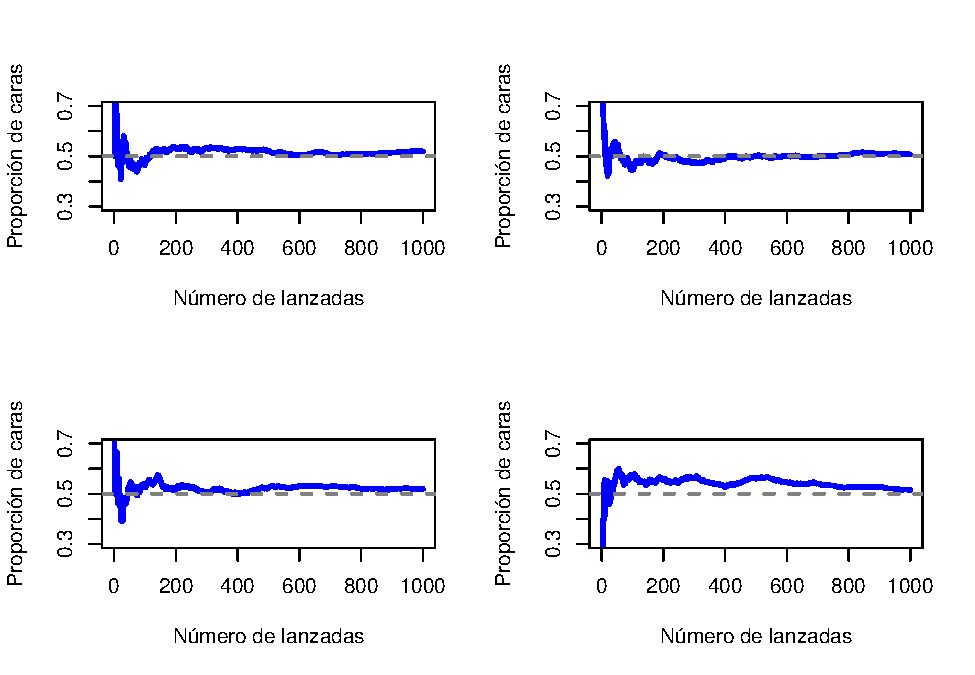
\includegraphics{FdI2_files/figure-latex/frequentistprobability-1.pdf}
\caption{\label{fig:frequentistprobability} Una imagen de cómo funciona la
probabilidad frecuentista. Si lanzas una moneda justa una y otra vez, la
proporción de caras deja de fluctuar y converge hacia la probabilidad
real de 0.5. Cada panel muestra uno de las cuatro simulaciones con 1.000
lanzamientos cada uno. Aunque ninguna de estas simulaciones terminó con
un valor exacto de .5, si hubiéramos extendido el experimento por un
número infinito de lanzamientos lo habríamos conseguido.}
\end{figure}

La definición frecuentista de probabilidad tiene algunas características
que le hacen deseable. En primer lugar, es objetivo: la probabilidad de
un evento se basa \emph{necesariamente} en el mundo real. La única forma
en que declaraciones de probabilidad puedan tener sentido es si se
refieren a (una secuencia de) eventos que ocurren en el universo físico.
En segundo lugar, es inequívoco: dos personas que miran como se
desarrolla la misma secuencia de eventos, al tratar de calcular la
probabilidad de un evento, inevitablemente deberán llegar a la misma
respuesta. Sin embargo, también tiene algunas características no tan
deseables. En primer lugar, no existen secuencias infinitas en el mundo
físico. Supongamos que has encontrado una moneda en el suelo y has
comenzado a lanzarla varias veces. Cada vez que aterriza, impacta en el
suelo. Cada impacto daña un poco la moneda; eventualmente, la moneda
será inutilizable. Entonces, uno podría preguntarse si realmente tiene
sentido fingir que una secuencia ``infinita'' de lanzamientos de monedas
es un concepto significativo u objetivo. No podemos decir que una
``secuencia infinita'' de eventos es algo real en el universo físico,
porque el universo físico no permite nada infinito. Así, podemos ver que
la definición frecuentista tiene un alcance limitado. Hay muchas cosas
por ahí a las que los seres humanos estamos felices de asignar
probabilidades en el día a día, pero que no pueden (ni siquiera en
teoría) ser planteadas como una secuencia hipotética de eventos. Por
ejemplo, si un meteorólogo aparece en televisión y dice: ``la
probabilidad de lluvia en Pamplona el 2 de noviembre del 2048 es del
60\%'' nosotros podemos aceptarlo sin rechistar. Pero desde un punto de
vista frecuentista, no queda tan claro cómo podemos definirlo. Sólo hay
una ciudad de Pamplona (en Navarra), y sólo un 2 de noviembre del 2048.
Aquí no hay una secuencia infinita de eventos, solo una cosa de una vez.
La probabilidad frecuentista nos \emph{prohíbe} hacer declaraciones de
probabilidad sobre un solo evento. Desde la perspectiva frecuentista,
lloverá mañana o o no lloverá; no hay una ``probabilidad'' que se pueda
adjuntar a un sólo evento no repetible. Sin embargo, existen algunos
trucos que los frecuentistas pueden utilizar para solucionar esta
situación. Una posibilidad es que el meteorólogo en realidad nos quiera
decir algo así: ``Existe una categoría de días para la que predigo un
60\% probabilidad de lluvia; si miramos sólo esos días para los que hago
esta predicción, entonces en el 60\% de esos días lloverá realmente''.
Es un poco extraño y contradictorio pensarlo de esta manera, pero los
frecuentistas hacen esto a veces.

\subsection{La visión bayesiana}\label{la-vision-bayesiana}

La alternativa a la visión frecuentista, la \textbf{\emph{visión
bayesiana}} de la probabilidad, a menudo se denomina visión
subjetivista, y es una visión relativamente minoritaria entre los
estadísticos, aunque ha ido ganando terreno constantemente a lo largo de
las últimas décadas. Hay muchos formas de bayesianismo, lo que hace
difícil decir exactamente cuál es ``la'' visión bayesiana. La forma más
fácil de entender la probabilidad subjetiva es al definir la
probabilidad de un evento como el \textbf{\emph{grado de creencia}} que
un agente inteligente y racional asigna a la verdad de ese evento. Desde
esa perspectiva, las probabilidades no existen en el mundo, sino más
bien en los pensamientos y suposiciones de las personas y otros seres
inteligentes. Sin embargo, para que este enfoque funcione, necesitamos
una forma de operacionalizar este ``grado de creencia''. Una forma de
hacerlo es formalizándolo en términos de una ``apuesta racional'' aunque
existen muchas otras formas. Supongamos que creo que existe una
probabilidad de que llueva mañana de un 60\%. Si alguien me hace una
apuesta, si llueve mañana, gano \$5, pero si no llueve, pierdo \$5.
Claramente, desde mi punto de vista, esta es una buena apuesta. Por otro
lado, si creo que la probabilidad de lluvia es sólo del 40\%, entonces
es una mala apuesta. Por lo tanto, podemos poner en práctica la noción
de una ``probabilidad subjetiva'' en términos de qué apuestas que estoy
dispuesto a aceptar.

¿Cuáles son las ventajas y desventajas del enfoque bayesiano? La
principal ventaja es que le permite asignar probabilidades a cualquier
evento. No esta limitado a aquellos eventos que son repetibles. La
principal desventaja (para muchas personas) es que no podemos ser
realmente objetivos - especificar una probabilidad requiere que
especifiquemos la entidad que tiene el grado de creencia que estamos
examinando. Esta entidad puede ser un humano, un extraterrestre, un
robot o incluso un estadístico, pero tiene que ser un agente inteligente
que sea capaz de creer en cosas. Para muchas personas esto representa un
inconveniente: parece hacer que la probabilidad sea arbitraria. Si bien
el enfoque bayesiano requiere que el agente en cuestión sea racional (es
decir, que obedezca las reglas de la probabilidad), permite que todos
tengan sus propias creencias; yo puedo creer que la moneda es justa
mientras que otro no, aunque ambos seamos racionales. La visión
frecuentista no permite que dos observadores atribuyan diferentes
probabilidades al mismo evento: cuando eso sucede, al menos uno de ellos
debe estar equivocado. La visión bayesiana no evita que esto ocurra. Dos
observadores con diferentes conocimientos previos pueden tener creencias
diferentes sobre el mismo evento. En otras palabras, mientras que la
visión frecuentista se puede considerar como demasiado estrecha (prohíbe
muchas cosas a las cuales queremos asignar probabilidades), la visión
bayesiana puede resultar demasiado amplia (permite demasiadas
diferencias entre observadores).

\subsection{¿Cuál es la diferencia? ¿Y quién tiene
razón?}\label{cual-es-la-diferencia-y-quien-tiene-razon}

Ahora que hemos visto ambas visiones estadísticas de forma
independiente, es necesario compararlas. Regresemos al hipotético juego
de fútbol de robots que comentamos comienzo del tema. ¿Que dirían un
frecuentista y un bayesiano sobre las tres afirmaciones? ¿Qué enunciado
sería la definición de probabilidad correcta para el frecuentista? ¿Y
para el bayesiano? ¿Es posible que alguno de los enunciados no tenga
sentido para cualquiera de los dos? Si entendemos ambas perspectivas,
podemos intuir cómo responder a estas preguntas.

Entendiendo las diferencias, podemos preguntarnos a continuación cuál de
dos enfoques es el \emph{correcto}. Sin embargo, no existe una respuesta
correcta. Matemáticamente hablando, no hay nada incorrecto sobre la
forma en que los frecuentistas piensan sobre secuencias de eventos, ni
hay nada incorrecto acerca de la forma en que los bayesianos definen las
creencias de un agente racional. De hecho, si vamos al detalle, los
bayesianos y los frecuentistas en realidad están de acuerdo en muchas
cosas. Muchos métodos frecuentistas conducen a decisiones que los
bayesianos pensarían que toma un agente racional. Muchos métodos
bayesianos tienen buenas propiedades frecuentistas.

En cualquier caso, la mayor parte de los métodos y análisis estadísticos
en la literatura se basan en el enfoque frecuentista. Por lo tanto, el
objetivo de esta asignatura es cubrir aproximadamente el mismo temario
que una clase típica de estadística de pregrado en ciencias de la
educación, y si queremos entender las herramientas estadísticas
utilizadas por la mayoría de los educadores en investigación,
necesitaremos una buena comprensión de los métodos frecuentistas.

\section{Teoría de probabilidad básica}\label{basicprobability}

A pesar de los argumentos ideológicos entre bayesianos y frecuentistas,
existe un consenso más o menos generalizado sobre las reglas que la
probabilidad debe obedecer. Hay muchas formas de abordar estas reglas.
El enfoque más utilizado se basa en el trabajo de Andrey Kolmogorov, uno
de los grandes matemáticos soviéticos del siglo XX. No entraremos mucho
en detalle, pero aprenderemos en qué consisten y cómo utilizarlas a
través del siguiente ejemplo.

\subsection{Introducción a las distribuciones de
probabilidad}\label{introduccion-a-las-distribuciones-de-probabilidad}

Un hecho comprobado sobre mi vida es que sólo tengo 5 pares de
pantalones: tres pares de vaqueros, los pantalones de un traje y un par
de pantalones de chándal. Lo más triste es que les he dado nombres: los
llamo \(X_1\), \(X_2\), \(X_3\), \(X_4\) y \(X_5\). Diariamente, por la
mañana, elijo un único par de esos pantalones que voy a usar. Si yo
tuviera que describir esta situación usando el lenguaje de la teoría de
la probabilidad, me referiría a cada par de pantalones (es decir, a cada
\(X\)) como un \textbf{\emph{evento elemental}}. La característica clave
de estos eventos elementales es que cada vez que hacemos una observación
(por ejemplo, cada vez que escojo un par de pantalones), el resultado
será uno y solo uno de estos eventos. Como he dicho antes, siempre uso
exactamente sólo un par de pantalones, así que mis pantalones cumplen
con esta restricción. Del mismo modo, al conjunto de todos los eventos
posibles se le denomina \textbf{\emph{espacio muestral}}. Siguiendo con
el ejemplo, mi espacio muestral sería el armario que contiene los 5
pantalones.

Bien, ahora que tenemos un espacio muestral (un armario), que está
construido a partir de muchas posibles eventos elementales (pantalones),
lo que queremos hacer es asignar una \textbf{\emph{probabilidad}} a cada
uno de estos eventos elementales. Para un evento \(X\), la probabilidad
de ese evento \(P(X)\) es un número que se encuentra entre 0 y 1. Cuanto
mayor sea el valor de \(P(X)\), más probable será que ocurra el evento.
Entonces, por ejemplo, si \(P(X) = 0\), significa que el evento \(X\) es
imposible (es decir, nunca uso esos pantalones). Por otro lado, si
\(P(X) = 1\) significa que el evento \(X\) es seguro que ocurra (es
decir, siempre uso esos pantalones). Los valores de probabilidad
intermedios, significan que a veces uso esos pantalones (y a veces no).
Por ejemplo, una \(P(X) = 0.5\) significa que uso esos pantalones la
mitad de las veces.

Llegados a este punto, lo siguiente que debemos entender es que ``algo
siempre sucede''. Cada vez que me pongo unos pantalones, realmente
termino usando esos pantalones. Lo que esto significa en términos
probabilísticos, es que las probabilidades de todos los eventos
elementales siempre suman 1. Esto se conoce como la \textbf{\emph{ley de
probabilidad total}}. Si se cumplen estos requisitos (tenemos número
\(X\) de pantalones, cada par con una probabilidad \(P(X)\) de usarlos
que en total suman 1), entonces lo que tenemos es una
\textbf{\emph{distribución de probabilidad}}.Veamos un ejemplo de
distribución de probabilidad

\begin{longtable}[]{@{}llllll@{}}
\toprule
Pantalones & V..azules & V..grises & V..negros & Traje.negro &
Chándal.azul\tabularnewline
\midrule
\endhead
Nombre & \(X_1\) & \(X_2\) & \(X_3\) & \(X_4\) & \(X_5\)\tabularnewline
Probabilidad & \(P(X_1) = .5\) & \(P(X_2) = .3\) & \(P(X_3) = .1\) &
\(P(X_4) = 0\) & \(P(X_5) = .1\)\tabularnewline
\bottomrule
\end{longtable}

Cada uno de estos eventos tiene una probabilidad que se encuentra entre
0 y 1, y si sumamos la probabilidad de todos eventos, suman 1. Incluso
podemos dibujar un gráfico de barras para visualizar esta distribución,
como se muestra en la Figura \ref{fig:pantsprob}.

\begin{figure}
\centering
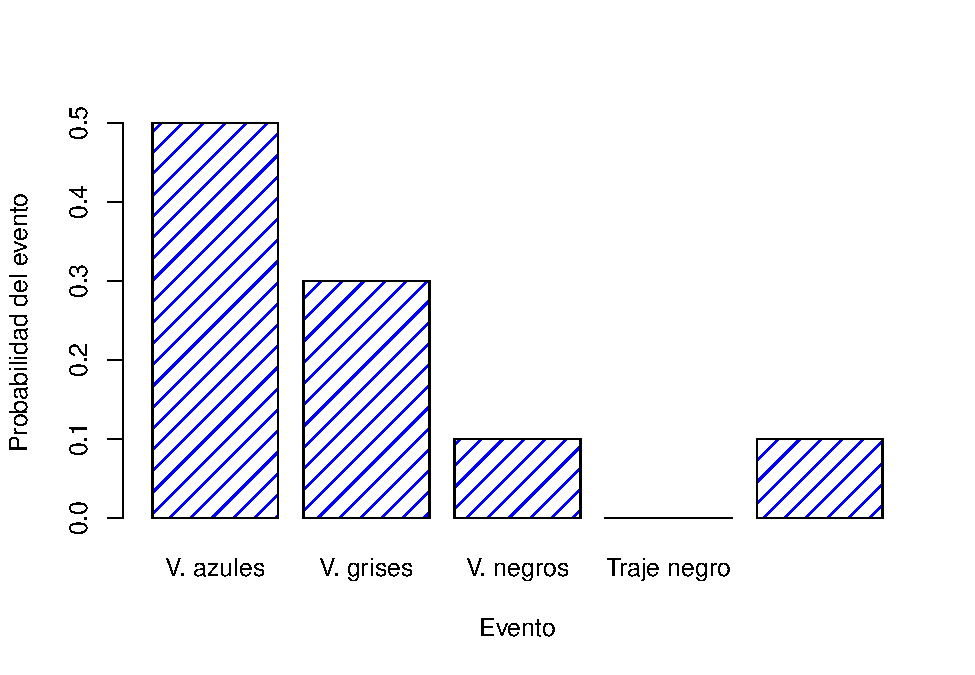
\includegraphics{FdI2_files/figure-latex/pantsprob-1.pdf}
\caption{\label{fig:pantsprob}Demostración visual de la distribución de
probabilidad de los ``pantalones''. Existen 5 ``eventos elementales'',
que se corresponden con mis 5 pares de pantalones. Cada evento tiene una
probabilidad de ocurrir: esta probabilidad es un número entre 0 y 1. La
suma de estas probabilidades es 1.}
\end{figure}

Es importante señalar que la teoría de probabilidades permite hablar
acerca de eventos elementales pero también sobre los
\textbf{\emph{eventos no elementales}}. La forma más fácil de ilustrar
este concepto es con un ejemplo. Siguiendo con el ejemplo de los
pantalones, es perfectamente posible hablar sobre la probabilidad de
usar vaqueros. Bajo esta premisa, podemos decir que el evento ``yo uso
vaqueros'' es posible siempre y cuando ocurra alguno de los eventos
elementales apropiados; en este caso ``vaqueros azules'', ``vaqueros
negros'' o ``vaqueros grises''. En términos matemáticos, definimos al
evento \(E\) ``vaqueros'' como el conjunto de eventos elementales
\((X_1, X_2, X_3)\). Si se produce alguno de estos eventos elementales,
también podemos decir que \(E\) ha ocurrido. Por lo tanto, podemos decir
que la probabilidad \(P(E)\) es simplemente la suma de esos tres
eventos, así \[
P(E) = P(X_1) + P(X_2) + P(X_3)
\] y, dado que las probabilidades de los vaqueros azules, grises y
negros son respectivamente .5, .3 y .1, la probabilidad total de usar
vaqueros es igual a .9.

Todo esto parece obvio y simple. Sin embargo, a partir de estos simples
comienzos, es posible construir algunas herramientas matemáticas más
complejas y poderosas. En la siguiente Tabla se muestran algunas de las
otras reglas que deben de cumplirse para poder calcular probabilidades.

\begin{longtable}[]{@{}llll@{}}
\toprule
Castellano & Notacion & Igual & Formula\tabularnewline
\midrule
\endhead
No \(A\) & \(P(\neg A)\) & = & \(1-P(A)\)\tabularnewline
\(A\) o \(B\) & \(P(A \cup B)\) & = &
\(P(A) + P(B) - P(A \cap B)\)\tabularnewline
\(A\) y \(B\) & \(P(A \cap B)\) & = &
\(P(A \vert B) P(B)\)\tabularnewline
\bottomrule
\end{longtable}

\section{La distribución binomial}\label{binomial}

Como hemos visto, las distribuciones de probabilidad pueden variar
enormemente, por lo que existe un gran número de distribuciones
posibles. Sin embargo, no todas son igual de importantes. Las
distribuciones más importantes, y de las que hablaremos en esta
asignatura son cinco: la distribución binomial, la distribución normal,
la distribución \(t\), la distribución \(\chi^2\) (``chi-cuadrada'') y
la distribución \(F\). Daremos una breve introducción a las cinco,
prestando especial atención a las distribuciones binomial y normal.
Comenzaremos con la distribución más simple de las cinco, la
distribución binomial.

\subsection{Introducción al binomio}\label{introduccion-al-binomio}

La teoría de la probabilidad se creó originalmente para intentar
describir cómo funcionaban los juegos de azar, por lo que parece
adecuado que nuestra discusión sobre la \textbf{\emph{distribución
binomial}} involucre una discusión sobre tirar dados y lanzar monedas.
Imaginemos el siguiente ``experimento'': tengo en mi poder 20 dados
iguales de seis caras. En una de las caras de cada dado hay una imagen
de una calavera; las otras cinco caras están en blanco. Si tiro los 20
dados, ¿cuál es la probabilidad de que obtenga exactamente 4 calaveras?
Asumiendo que los dados son justos, sabemos que la probabilidad de que
en un dado salga la calavera es de de 1 en 6; dicho de otra forma, la
probabilidad de que salga calavera en un solo dado es de aproximadamente
\(.167\). Esta información es suficiente para poder responder a nuestra
pregunta anterior, así que veamos cómo hacerlo.

Primero, pondremos algunos nombres a los eventos con su respectiva
notación. Dejaremos que \(N\) denote el número de dados que se tiran en
nuestro experimento; a esto se le conoce como el \textbf{\emph{parámetro
de tamaño}} de nuestra distribución binomial. También usaremos
\(\theta\) para referirnos a la probabilidad de que al tirar un solo
dado salga calavera, una cantidad que generalmente se denomina como la
\textbf{\emph{probabilidad de éxito}} del binomio.\footnote{Hay que
  tener en cuenta que el término ``éxito'' es bastante arbitrario, y en
  realidad no implica que el resultado sea algo deseado. Si \(\theta\)
  se refiriera a la probabilidad de que un pasajero se lesione en un
  accidente de autobús, seguiría siendo una probabilidad de éxito,
  aunque en realidad no queremos que la gente salga lastimada}
Finalmente, usaremos \(X\) para referirnos a los resultados de nuestro
experimento, es decir, la cantidad de calaveras que obtengo cuando lanzo
los dados. Dado que el valor real de \(X\) se debe al azar, nos podemos
referir a ella como una \textbf{\emph{variable aleatoria}}. En cualquier
caso, ahora que tenemos toda esta terminología y notación, podemos
utilizarlos para exponer el problema que planteábamos en el párrafo
anterior con mayor precisión. La cantidad que queremos calcular es la
probabilidad de que \(X = 4\) sabiendo que \(\theta = .167\) y \(N=20\).
La ``forma'' general de esta probabilidad que me interesa calcular
podría escribirse como, \[
  P(X \ | \ \theta, N)
\] donde estamos interesados en el caso específico donde \(X=4\),
\(\theta = .167\) y \(N=20\). Hace falta un elemento de notación más
antes de continuar con la solución del problema. Si yo quiero decir que
\(X\) se genera aleatoriamente a partir de una distribución binomial con
los parámetros \(\theta\) y \(N\), la notación que usaría para
expresarlo sería la siguiente: \[
  X \sim \mbox{Binomial}(\theta, N)
\]

Aunque no utilizaremos las fórmulas para hacer cálculos formalmente,
dejaré la fórmula de la distribución binomial en la Tabla
\ref{tab:distformulas}, ya que puede ser útil si se quieren entender
temas más avanzados con algo de profundidad. Por lo pronto, analizaremos
como se ve una distribución binomial (puedes hacerlo tú mismo si entras
\href{https://leudave.shinyapps.io/distribuciones/}{aquí}). La Figura
\ref{fig:binomial1} dibuja la probabilidad binomial para todos los
valores posibles de \(X\) de nuestro experimento de lanzamiento de
dados, partiendo desde \(X=0\) (ninguna sale calavera) hasta \(X=20\)
(salen todas calaveras). Hay que tener en cuenta que esto es básicamente
un gráfico de barras, al igual que la gráfica de la ``probabilidad de
pantalones'' de la Figura \ref{fig:pantsprob}. En el eje horizontal
tenemos todos los eventos posibles, y en el eje vertical podemos leer la
probabilidad de que ocurra cada uno de esos eventos. Por lo tanto, la
probabilidad de que salgan 4 calaveras al tirar 20 dados es de
aproximadamente 0,20 (la respuesta exacta es 0,2022036, como veremos en
un momento). En otras palabras, esperaría que ese evento suceda
aproximadamente el 20\% de las veces que se lleve a cabo este
experimento.

\begin{table}[t]

\caption{\label{tab:distformulas}Fórmulas para las distribuciones binomial y normal. En la ecuación de la binomial, $X!$ es una función factorial (es decir, multiplica todos los números enteros de  1 hasta $X$), y en la de la distribución normal "exp" se refiere a una función exponencial.}
\centering
\begin{tabular}{l|l}
\hline
Binomial & Normal\\
\hline
\$P(X | \textbackslash{}theta, N) = \textbackslash{}displaystyle\textbackslash{}frac\{N!\}\{X! (N-X)!\}  \textbackslash{}theta\textasciicircum{}X (1-\textbackslash{}theta)\textasciicircum{}\{N-X\}\$ & \$p(X | \textbackslash{}mu, \textbackslash{}sigma) = \textbackslash{}displaystyle\textbackslash{}frac\{1\}\{\textbackslash{}sqrt\{2\textbackslash{}pi\}\textbackslash{}sigma\} \textbackslash{}exp \textbackslash{}left( -\textbackslash{}frac\{(X - \textbackslash{}mu)\textasciicircum{}2\}\{2\textbackslash{}sigma\textasciicircum{}2\} \textbackslash{}right)\$\\
\hline
\end{tabular}
\end{table}

\begin{figure}
\centering
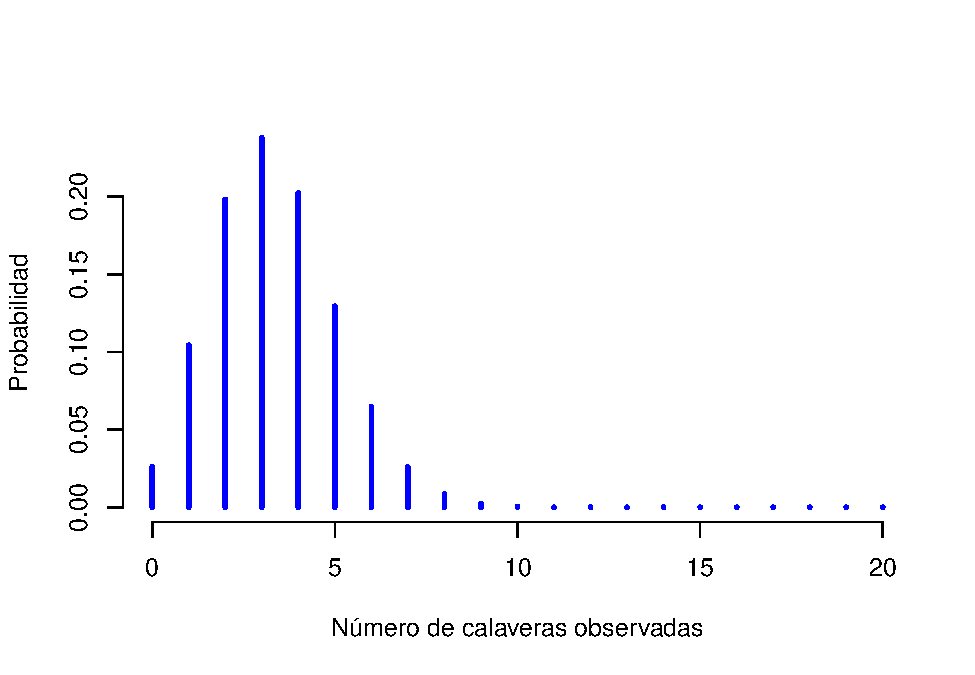
\includegraphics{FdI2_files/figure-latex/binomial1-1.pdf}
\caption{\label{fig:binomial1} La distribución binomial con parámetro de
tamaño de \(N=20\) y una probabilidad de éxito de \(theta = 1/6\). Cada
barra vertical representa la probabilidad de un resultado específico (un
valor posible de \(X\)). Ya que esta es una distribución de
probabilidad, cada una de las probabilidades debe ser un número entre 0
y 1, y la altura de las barras también deben sumar 1.}
\end{figure}

Para darte una idea de cómo cambia la distribución binomial cuando
modificamos los valores de \(\theta\) y \(N\), supongamos que en lugar
de tirar dados, en realidad estoy lanzando monedas. Esta vez, mi
experimento implica lanzar una moneda justa repetidamente, y el
resultado que me interesa es la cantidad de caras que observo. En este
escenario, la probabilidad de éxito ahora es de \(\theta = 1/2\).
Supongamos que tirara la moneda \(N=20\) veces. En este ejemplo, he
cambiado la probabilidad de éxito, pero mantuve el tamaño de la muestra
del experimento. ¿Qué efecto tiene este cambio en nuestra distribución
binomial? Bueno, como la Figura \ref{fig:binomial2a} muestra, el efecto
principal fue el desplazamiento de toda la distribución hacia la
derecha, como era de esperar. ¿Y si lanzamos una moneda \(N=100\) veces?
En este caso obtendremos algo como lo de la Figura \ref{fig:binomial2b}.
La distribución se mantiene aproximadamente en el medio, pero hay un
poco más de variabilidad en los posibles resultados.

\begin{figure}
\centering
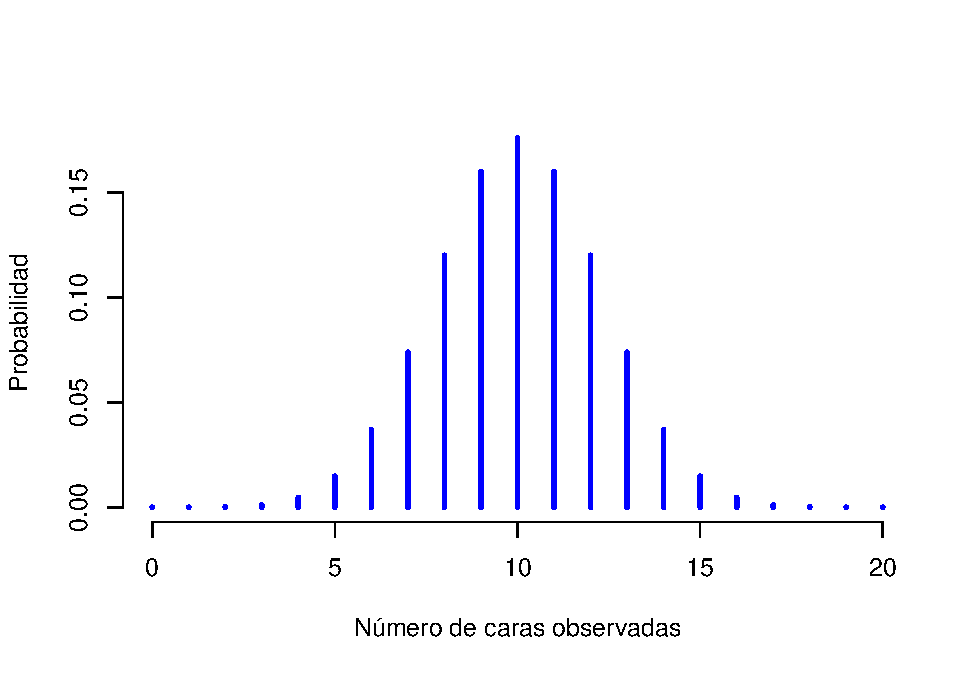
\includegraphics{FdI2_files/figure-latex/binomial2a-1.pdf}
\caption{\label{fig:binomial2a}Dos distribuciones binomiales, que involucran
un escenario en el que lanzo una moneda justa, donde la probabilidad de
éxito es \(theta = 1/2\). Asumimos que estoy lanzando la moneda \(N=20\)
veces.}
\end{figure}

\begin{figure}
\centering
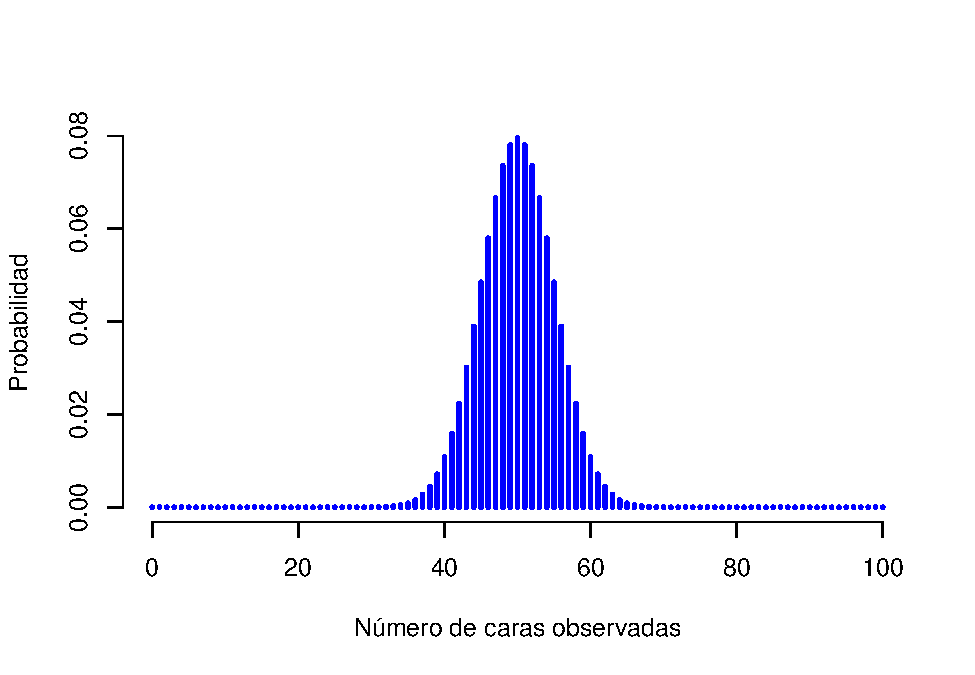
\includegraphics{FdI2_files/figure-latex/binomial2b-1.pdf}
\caption{\label{fig:binomial2b}Dos distribuciones binomiales, que involucran
un escenario en el lanzo una moneda justa, donde la probabilidad de
éxito subyacente es \(theta = 1/2\). Asumimos que estoy lanzando la
moneda \(N=100\) veces.}
\end{figure}

\section{La distribución normal}\label{normal}

Si bien la distribución binomial es conceptualmente la distribución más
sencilla de entender, no es la más importante. Ese honor le corresponde
a la \textbf{\emph{distribución normal}}, también conocida como ``curva
de campana'' o como ``distribución gaussiana'' o ``campana de Gauss''.
Una distribución normal se describe utilizando dos parámetros, la media
de la distribución \(\mu\) y la desviación estándar de la distribución
\(\sigma\). La notación que utilizamos para decir que una variable \(X\)
se distribuye normalmente es la siguiente:

\[
  X \sim \mbox{Normal}(\mu,\sigma)
\] Al igual que con la distribución binomial, he incluido la fórmula
para la distribución normal en la tabla \ref{tab:distformulas}, porque
creo que es lo suficientemente importante como para que todos los que
aprenden algo de estadística al menos la conozcan, aunque no nos
enfoquemos en ella.

Vamos intentar descifrar lo que significa que una variable esté
normalmente distribuida. Echemos un vistazo a la Figura
\ref{fig:normdist}, que muestra una distribución normal con media
\(\mu = 0\) y desviación estándar \(\sigma = 1\). Con un poco de
imaginación, podemos apreciar de dónde viene el nombre ``curva de
campana''. A diferencia de los gráficos sobre la distribución binomial,
la imagen de la distribución normal en la Figura \ref{fig:normdist}
muestra una curva suave en lugar de barras ``tipo histograma''. Esto no
es arbitrario: la distribución normal es continua, mientras que la
distribución binomial es discreta. Por ejemplo, en el experimento de
tiro de dados de la sección anterior, es posible obtener 3 calaveras o 4
calaveras, mientras que un valor intermedio como 3.9 es imposible de
obtener. Este hecho se ve reflejado en la Figura \ref{fig:binomial1},
donde tenemos una barra ubicada en \(X=3\) y otra en \(X=4\), pero entre
ellas no hay nada. En cambio, los valores continuos no tienen esta
restricción. Por ejemplo, supongamos que estamos hablando del tiempo. La
temperatura de un día primavera podría ser de 23 grados, 24 grados, 23.9
grados o cualquier cosa intermedia, ya que la temperatura es una
variable continua, por lo que una distribución normal podría ser la
herramienta apropiada para describir las diferentes temperaturas en los
días de primavera.\footnote{En la práctica, la distribución normal es
  tan útil que las personas tienden a usarla incluso cuando la variable
  no es continua. Siempre que haya suficientes categorías (por ejemplo,
  respuestas de escala Likert de un cuestionario), suele ser frecuente
  el uso de la distribución normal.}

\begin{figure}
\centering
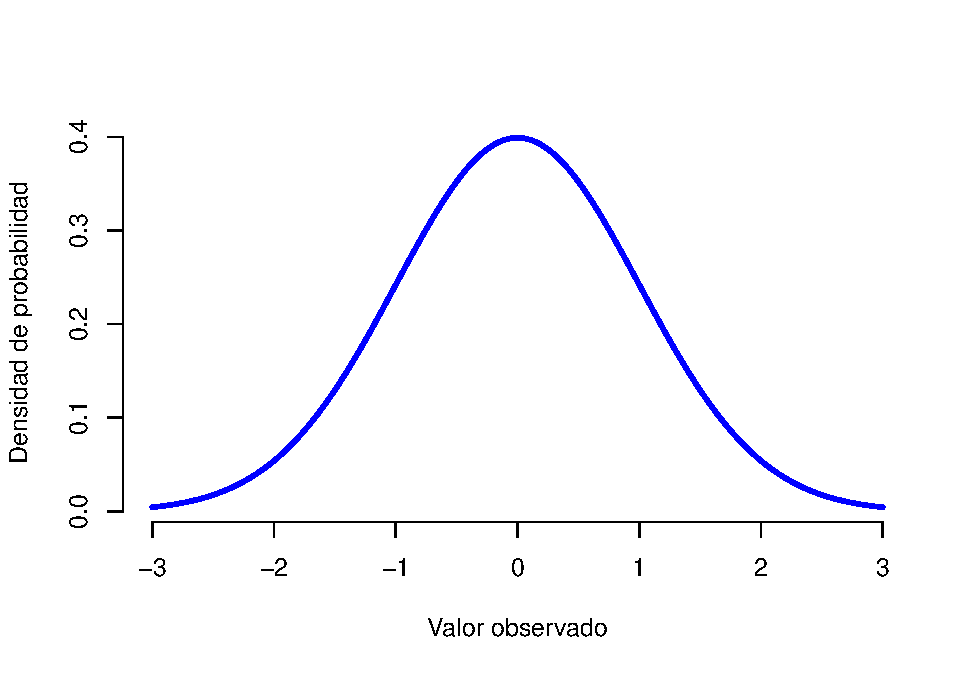
\includegraphics{FdI2_files/figure-latex/normdist-1.pdf}
\caption{\label{fig:normdist} Distribución normal con media \(mu = 0\) y
desviación estándar \(sigma = 1\). El eje \(x\) corresponde con el valor
de alguna variable, y el eje \(y\) nos dice qué tan probable es que
observemos ese valor. Sin embargo, vemos como el eje \(y\) se denomina
``Densidad de Probabilidad'' y no ``Probabilidad''. La altura de la
curva no representa como tal la probabilidad de observar un valor
particular de \(x\). Sin embargo, las alturas nos informan sobre qué
valores de \(x\) son más probables (¡los más altos!).}
\end{figure}

Una vez visto esto, vamos a analizar cómo funciona una distribución
normal. En primer lugar, veamos qué es lo que sucede cuando jugamos con
los parámetros de la distribución (puedes hacerlo tú mismo si entras en
este enlace). La Figura \ref{fig:normmean} muestra distribuciones
normales que tienen medias diferentes, pero con la misma desviación
estándar. Como es de esperar, todas estas distribuciones tienen la misma
``anchura''. La unica diferencia entre ellas es que se han desplazado
hacia la izquierda o hacia la derecha. En todos los demás aspectos son
idénticas. Por el contrario, si aumentamos la desviación estándar
mientras mantenemos la media constante, el pico de la distribución
permanece en el mismo lugar, pero la distribución se amplía, como
podemos ver en la Figura \ref{fig:normsd}. Sin embargo, cuando ampliamos
la distribución, la altura del pico disminuye. Esto \emph{tiene} que
suceder: de la misma forma que las alturas de las barras de una
distribución binomial discreta tienen que \emph{sumar} 1, el total del
\emph{área bajo la curva} de una distribución normal debe ser igual a 1.

\begin{figure}
\centering
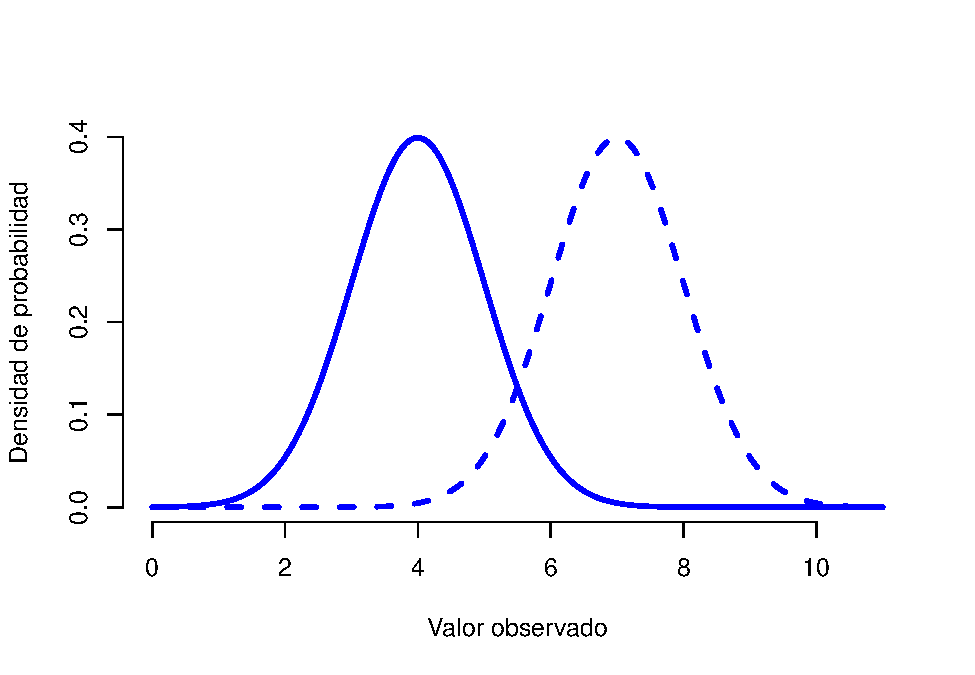
\includegraphics{FdI2_files/figure-latex/normmean-1.pdf}
\caption{\label{fig:normmean}Gráfica que demuestra lo que sucede cuando se
cambia la media de una distribución normal. La línea sólida representa
una distribución normal con media de \(mu=4\). La línea discontinua
muestra una distribución normal con una media de \(mu=7\). En ambos
casos, la desviación estándar es de \(sigma=1\). Vemos como las dos
distribuciones tienen la misma forma, pero la distribución con la línea
discontinua se desplaza hacia la derecha.}
\end{figure}

\begin{figure}
\centering
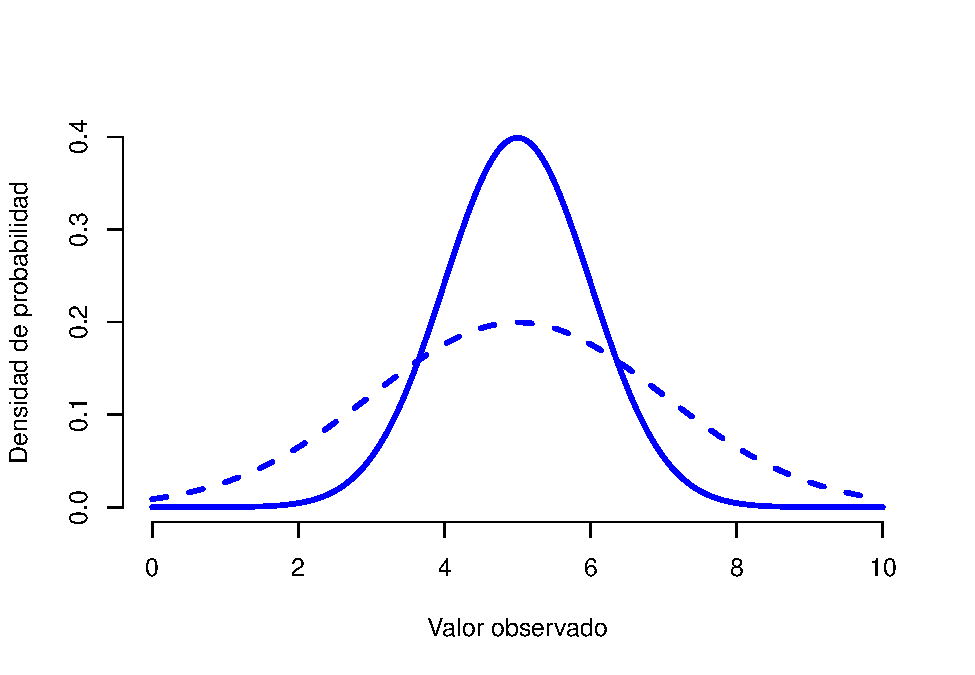
\includegraphics{FdI2_files/figure-latex/normsd-1.pdf}
\caption{\label{fig:normsd}Una ilustración de lo que sucede cuando cambia la
desviación estándar de una distribución normal. Ambas distribuciones
tienen una media de \(mu=5\), pero diferentes desviaciones estándar. La
línea continua dibuja una distribución con una desviación estándar
\(sigma=1\), y la línea discontinua muestra una distribución con
desviación estándar de \(sigma=2\). Como consecuencia, ambas
distribuciones están centradas en el mismo lugar, pero la distribución
con la línea discontinua es más ancha que la otra.}
\end{figure}

Antes de seguir adelante, quiero señalar una característica importante
de la distribución normal. Independientemente de los valores de la media
y la desviación estándar, un 68.3\% del área de la curva cae dentro de 1
desviación estándar sobre la media. Del mismo modo, el 95.4\% de la
distribución cae dentro de 2 desviaciones estándar sobre la media, y el
99.7\% de la distribución está dentro de 3 desviaciones estándar. Esta
idea se ilustra en las Figuras \ref{fig:sdnorm1} y \ref{fig:sdnorm2}.

\begin{figure}
\centering
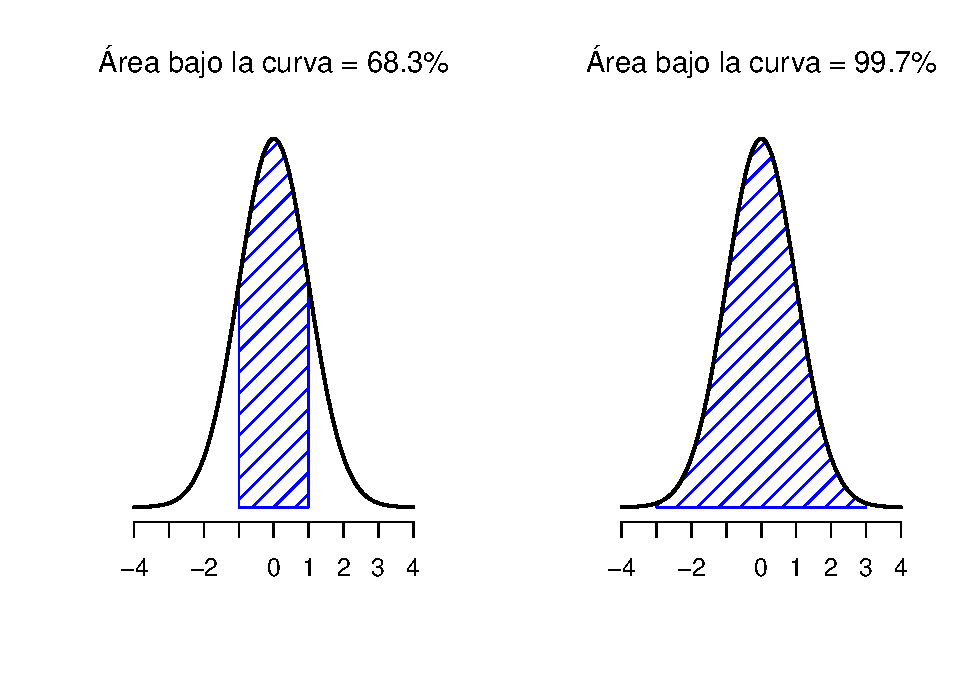
\includegraphics{FdI2_files/figure-latex/sdnorm1-1.pdf}
\caption{\label{fig:sdnorm1}El área bajo la curva indica la probabilidad de
que una observación se encuentre dentro de un rango determinado. Las
línea continua traza una distribución normal con media \(mu=0\) y
desviación estándar \(sigma=1\). El área sombreada ilustra el `área bajo
la curva' para dos casos importantes. En el panel a, podemos ver que hay
es un 68.3\% de probabilidad de que una observación caiga dentro de 1
desviación estándar sobre la media. En el panel b, vemos que existe una
probabilidad del 95.4\% de que una observación se encuentre dentro de 2
desviaciones estándar sobre la media.}
\end{figure}

\begin{figure}
\centering
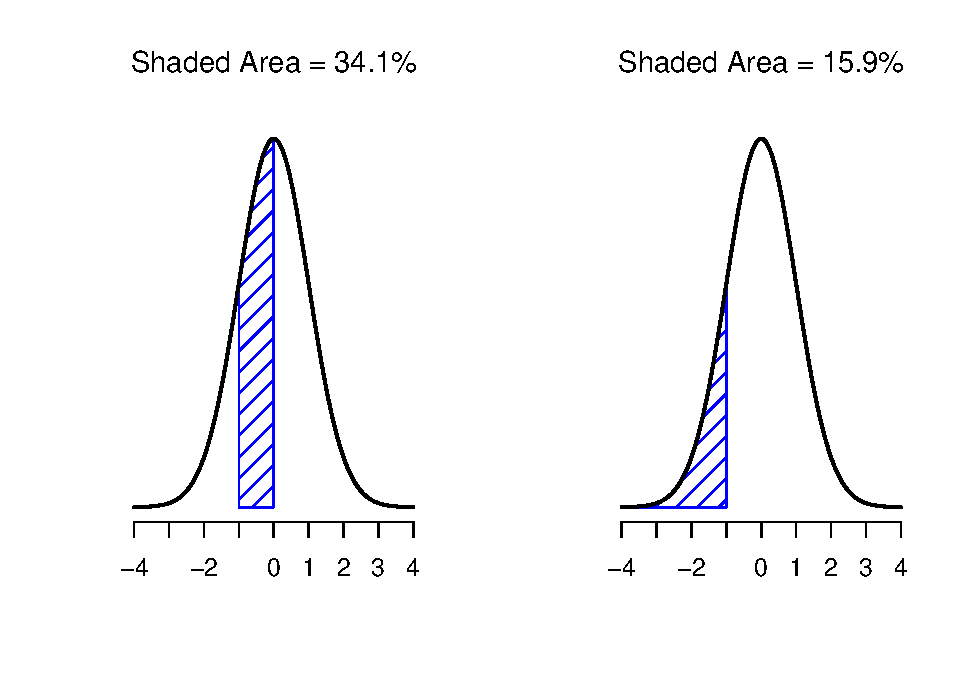
\includegraphics{FdI2_files/figure-latex/sdnorm2-1.pdf}
\caption{\label{fig:sdnorm2}Dos ejemplos más sobre el concepto del `área
bajo la curva'. Existe un 15.9\% de probabilidad de que una observación
se encuentre 1 desviación estándar o menos por debajo de la media (panel
a), y una probabilidad del 34.1\% de que una observación sea mayor que
una desviación estándar por debajo de la media pero menor que la media
(panel b). Si sumamos estos dos valores, obtendremos 15.9\% + 34.1\% =
50\%. Para datos que estén normalmente distribuidos, existe un 50\% de
probabilidad de que una observación caiga por debajo de la media. Esto
implica que existe un 50\% de probabilidad de que caiga por encima de la
media.}
\end{figure}

\subsection{Densidad de probabilidad}\label{density}

A lo largo de la discusión sobre la distribución normal, ha habido un
par de cosas que parecen no tener sentido. Quizás hayas notado que el
eje \(y\) en estas Figuras se denomina como ``Densidad de probabilidad''
en lugar de ``Probabilidad''. Tal vez notaste que utilizamos \(p(X)\) en
lugar de \(P(X)\) en la fórmula de la distribución normal.

Si utilizamos la Figura y calculamos (siguiendo la fórmula) la
probabilidad de \texttt{x\ =\ 1}, para una variable normalmente
distribuida con \texttt{media\ =\ 1} y desviación estándar
\texttt{sd\ =\ 0.1}, nos arrojará como resultado una probabilidad de
3.99. Sin embargo, hemos visto anteriormente que las probabilidades
\emph{no} pueden ser mayores que 1. Entonces, ¿qué es lo que hemos
calculado?

Lo que hemos calculado aquí en realidad no es una probabilidad: Para
entender qué es ese algo, tenemos que pensar qué es lo que realmente
\emph{significa} decir que \(X\) es una variable continua. Digamos que
estamos hablando de la temperatura otra vez. El termómetro me dice que
hacen 23 grados, pero yo sé que eso no es del todo cierto. No hacen 23
grados \emph{exactamente}. Quizás sea algo más cercano a los 23.1 grados
o, si seguimos, en realidad podrían ser 23.095 grados. Esto es lo que
sucede con los valores continuos: nunca se sabe el valor exacto.

Ahora pensemos en lo que esto implica cuando hablamos de probabilidades.
Supongamos la temperatura máxima para mañana se toma de una distribución
normal con media 23 y desviación estándar 1. ¿Cuál es la probabilidad de
que la temperatura sea \emph{exactamente} 23 grados? La respuesta es
``cero'', o posiblemente, ``un número tan cercano a cero que bien podría
ser cero''. ¿Por qué es esto? Es como intentar tirar un dardo en un
tablero de dardos con dianas infinitamente cada vez más pequeñas: no
importa cuán buena sea tu puntería, nunca acertarás. En la vida real
nunca obtendremos el valor exacto de 23. Siempre será 23.1 o 22.99998 o
algo así. En en otras palabras, no tiene sentido hablar de la
probabilidad de que la temperatura sea exactamente 23 grados. Sin
embargo, en el día a día, si el termómetro indica 23 grados pero en
realidad hacen 22.9998 grados, probablemente no nos importe demasiado.
Esto es porque en el día a día, ``23 grados'' por lo general significa
algo así como ``en algún lugar entre 22.5 y 23.5 grados''. Y aunque no
parezca muy importante preguntar por la probabilidad de que la
temperatura sea exactamente 23 grados, lo que sí lo parece es preguntar
sobre la probabilidad de que la temperatura se encuentre entre 22.5 y
23.5, o entre 20 y 30, o cualquier otro rango de temperaturas en el que
estemos interesados.

El objetivo de esta explicación es dejar claro que, cuando hablamos de
distribuciones continuas, no tiene sentido hablar sobre la probabilidad
de un valor específico. Sin embargo, sí que \emph{podemos} hablar sobre
la probabilidad de que el valor se encuentre dentro de un rango
particular de valores. Para encontrar probabilidad asociada con un rango
particular, lo que debe hacer es calcular el ``área bajo la curva''.
Este concepto lo conocemos: en la Figura \ref{fig:sdnorm1}, las áreas
sombreadas representan probabilidades genuinas (por ejemplo, la Figura
\ref{fig:sdnorm1} muestra la probabilidad de observar un valor que cae
dentro de 1 desviación estándar sobre la media).

Para finalizar, volveremos con la fórmula para \(p(x)\) que vimos
anteriormente. Los resultados de \(p(x)\) no describe una probabilidad,
sino una \textbf{\emph{densidad de probabilidad}}, que en las gráficas
corresponde a la altura de la curva. De la misma forma en que las
probabilidades son números no-negativos que deben sumar 1, las
densidades de probabilidad son números no-negativos que deben integrar a
1 (donde la integral se toma a través de todos los valores posibles de
\(X\)). Para calcular la probabilidad de que \(X\) caiga entre \(a\) y
\(b\) calculamos la integral definida de la función de densidad sobre el
rango correspondiente, \(\int_a^b p(x) \ dx\). Se trata simplemente de
otra forma de llegar al mismo resultado.

\section{Otras distribuciones útiles}\label{otherdists}

La distribución normal es la distribución más utilizada por los
estadísticos (por razones que se discutirán más adelante), y la
distribución binomial es útil muchos escenarios. Sin embargo, existen
otros tipos de distribuciones de probabilidad. Revisaremos brevemente 3
de ellas: la distribución \(t\), la distribución \(\chi^2\) y la
distribución \(F\). La \textbf{\emph{distribución \(t\)}} es una
distribución continua que se parece mucho a una distribución normal,
pero que tiene colas más pesadas (ver Figura \ref{fig:tdist}). Esta
distribución tiende a surgir en situaciones en las que piensa que los
datos siguen una distribución normal, pero no se conoce la media o la
desviación estándar.

\begin{figure}
\centering
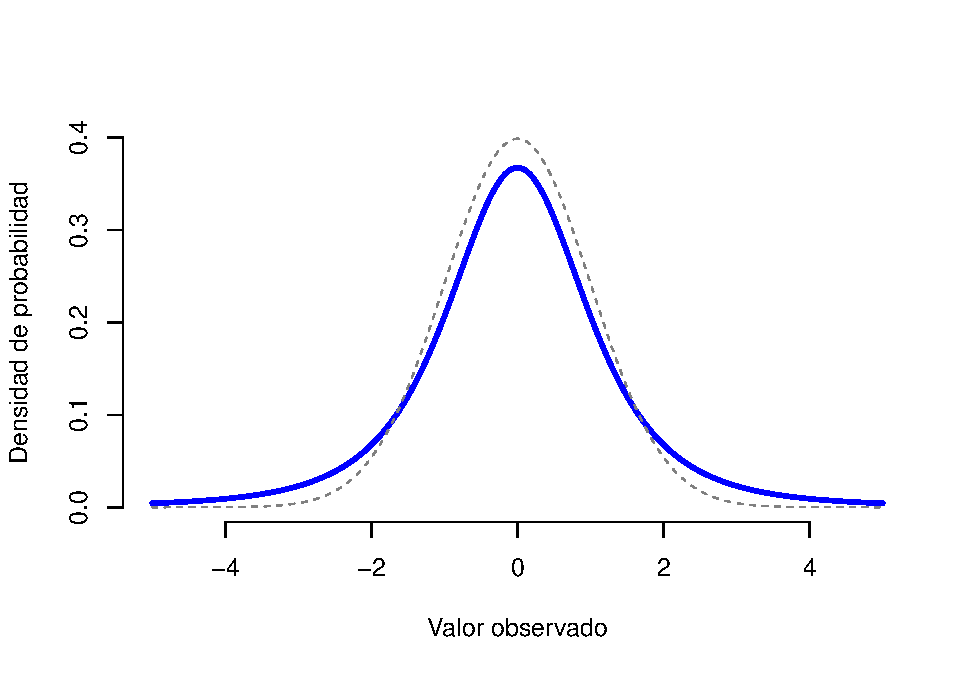
\includegraphics{FdI2_files/figure-latex/tdist-1.pdf}
\caption{\label{fig:tdist}Una distribución \(t\) con 3 grados de libertad
(línea continua). Se asemeja a una distribución normal, pero no es igual
(línea discontinua). Ten en cuenta que las ``colas'' de la distribución
\(t\) son más ``pesadas'' (es decir, se extienden más hacia afuera,
conteniendo más valores que se alejan de la media) que las colas de la
distribución normal.}
\end{figure}

\begin{itemize}
\tightlist
\item
  La \textbf{\emph{distribución \(\chi^2\)}} es otra distribución que
  podemos encontrar con cierta frecuencia. Es habitual encontrarla
  cuando hacemos análisis de datos categóricos. Los valores de una
  distribución \(\chi^2\) se consiguen al elevar al cuadrado los valores
  de una variable distribuída normalmente y luego sumarlos (un
  procedimiento denominado ``suma de cuadrados''). Después veremos
  porqué es útil hacer una ``suma de cuadrados''. La apariencia de una
  distribución \(\chi^2\) la puedes encontrar en la Figura
  \ref{fig:chisqdist}.
\end{itemize}

\begin{figure}
\centering
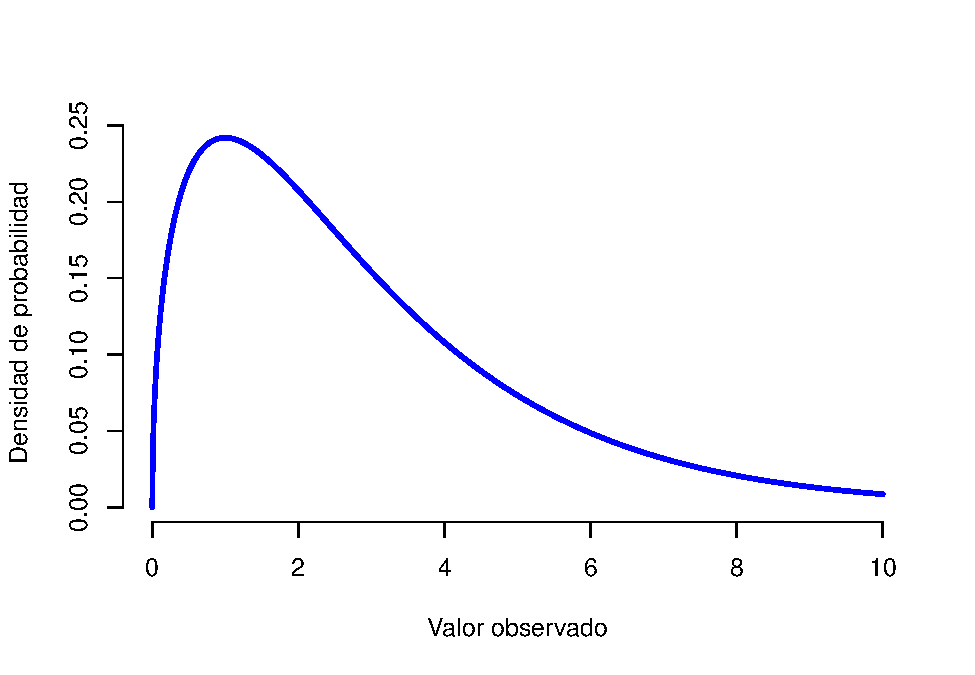
\includegraphics{FdI2_files/figure-latex/chisqdist-1.pdf}
\caption{\label{fig:chisqdist}Una distribución \(chi^2\) con 3 grados de
libertad (3 repeticiones, lo explicaremos más adelante). Observa que los
valores siempre deben ser mayores que cero (los valores se elevan al
cuadrado y se suman), y que la distribución es bastante sesgada (en este
caso hacia la derecha). Estas son las características clave de una
distribución chi-cuadrado.}
\end{figure}

\begin{itemize}
\tightlist
\item
  La \textbf{\emph{distribución \(F\)}} se parece un poco a la
  distribución \(\chi^2\) y surge cada vez que necesitamos comparar dos
  distribuciones \(\chi^2\) entre sí. Es decir, si queremos comparar dos
  ``sumas de cuadrados'' diferentes, nos encontraremos con una
  distribución \(F\). Aún no hemos visto un ejemplo de todo lo que
  implica una suma de cuadrados, pero lo veremos cuando hablemos sobre
  ANOVAs, donde nos encontraremos nuevamente con la distribución \(F\).
\end{itemize}

\begin{figure}
\centering
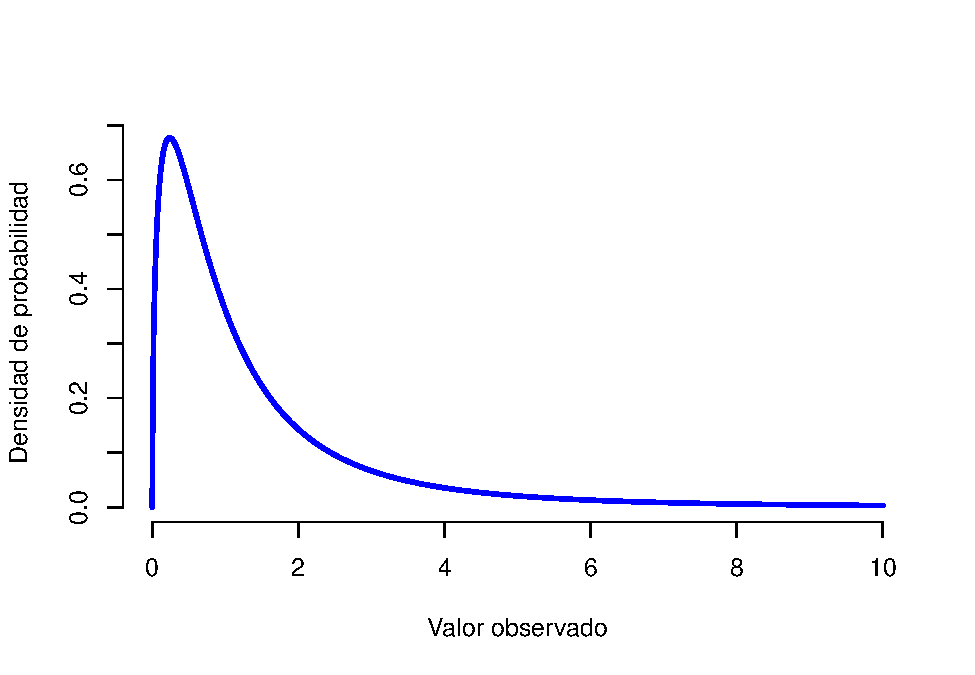
\includegraphics{FdI2_files/figure-latex/Fdist-1.pdf}
\caption{\label{fig:Fdist}Una distribución \(F\) con 3 y 5 grados de
libertad. Cualitativamente hablando, es similar a una distribución de
chi-cuadrado, pero por lo general el significado no es el mismo.}
\end{figure}

Debido a que estas distribuciones están estrechamente relacionadas con
la distribución normal y entre sí, y porque se convertirán en las
distribuciones importantes al hacer análisis estadísticos inferenciales
en este curso, creo que es útil hacer una pequeña demostración de cómo
estas distribuciones realmente están relacionadas entre sí. Primero,
imagina que tenemos un conjunto de 1,000 observaciones aleatorias
distribuidas normalmente al cual llamaremos ``Muestra A''.

Esta ``Muestra A'' es una variable que contiene 1,000 números que se
distribuyen normalmente y tienen una media de 0 y desviación estándar de
1. En la Figura \ref{fig:distnormal} podemos ver un histograma con la
distribución de los valores organizados por columnas, así como una línea
negra sólida que representa la distribución verdadera de los datos (es
decir, una distribución normal con valores infinitos con media 0 y
desviación estándar 1). Así podemos comparar los datos recién generados
con los de una distribución normal verdadera.

\begin{figure}
\centering
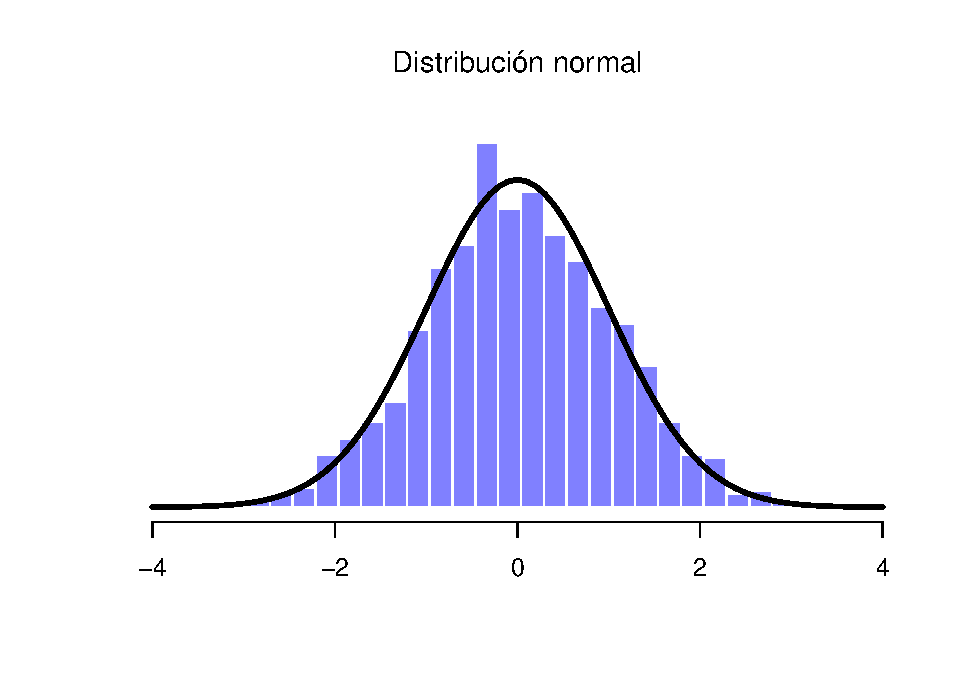
\includegraphics{FdI2_files/figure-latex/distnormal-1.pdf}
\caption{\label{fig:distnormal}Distribución normal de la Muestra A
(histograma), junto con la distribución normal verdadera (línea sólida)}
\end{figure}

En la Figura anterior podemos observar cómo han sido generados muchos
valores distribuidos normalmente que luego han sido comparados con la
distribución de probabilidad verdadera (línea sólida). Supongamos que
ahora queremos una distribución chi-cuadrada con 3 grados de libertad.
Como hemos mencionado anteriormente, una distribución chi-cuadrada con
\(k\) grados de libertad es es el resultado de tomar \(k\) variables (o
muestras) normalmente distribuidas (con media 0 y desviación estándar
1), elevarlas al cuadrado y sumarlas. Como queremos una distribución de
chi-cuadrada con 3 grados de libertad, además de nuestra ``Muestra A'',
necesitamos dos conjuntos más de valores (también distribuidos
normalmente). A estas nuevas dos variables las llamaremos ``Muestra B''
y ``Muestra C'':

\begin{figure}
\centering
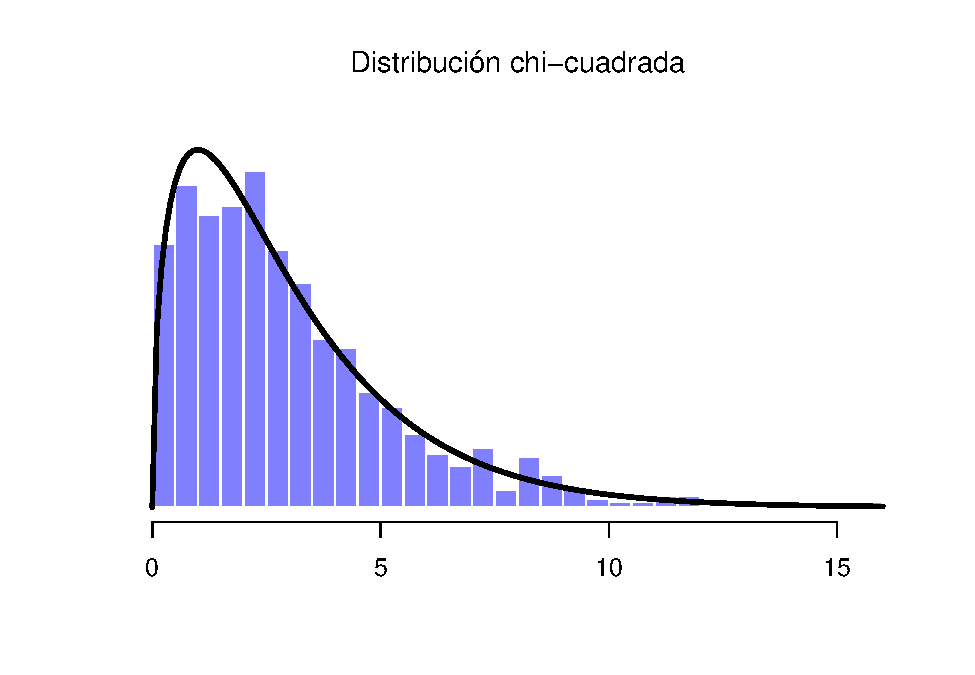
\includegraphics{FdI2_files/figure-latex/distchi-1.pdf}
\caption{\label{fig:distchi}Distribución chi-cuadrada. Incluye a las
Muestras A, B y C (3 grados de libertad)}
\end{figure}

Una vez que tenemos las tres variables, la teoría dice que debemos
elevarlos al cuadrado y sumarlos, con lo que obtendremos 1,000
observaciones que siguen una distribución de chi-cuadrada con 3 grados
de libertad. Visualmente, obtendremos una distribución como en la Figura
\ref{fig:distchi}.

Podemos extender esta demostración y tratar de entender el origen de la
distribución \(t\) y la distribución \(F\). Antes, hemos dicho que la
distribución \(t\) está relacionada con la distribución normal cuando se
desconoce la media o la desviación estándar. Sin embargo, existe una
relación más precisa entre las distribuciones normal, chi-cuadrada y
\(t\). Supongamos que ``escalamos'' nuestros datos anteriores de la
chi-cuadrada al dividirla entre sus 3 grados de libertad.

Si tomamos un conjunto de variables normalmente distribuidas (pensemos
ahora en una ``Muestra D'') y las dividimos por (la raíz cuadrada de)
nuestra variable chi-cuadrada ``escalada'' que tenía \(k=3\) grados de
libertad, la operación dará como resultado una distribución \(t\) con 3
grados de libertad. Si trazamos el histograma de esta nueva distribución
\(t\), observaremos algo parecido al de la Figura \ref{fig:distt}.

\begin{figure}
\centering
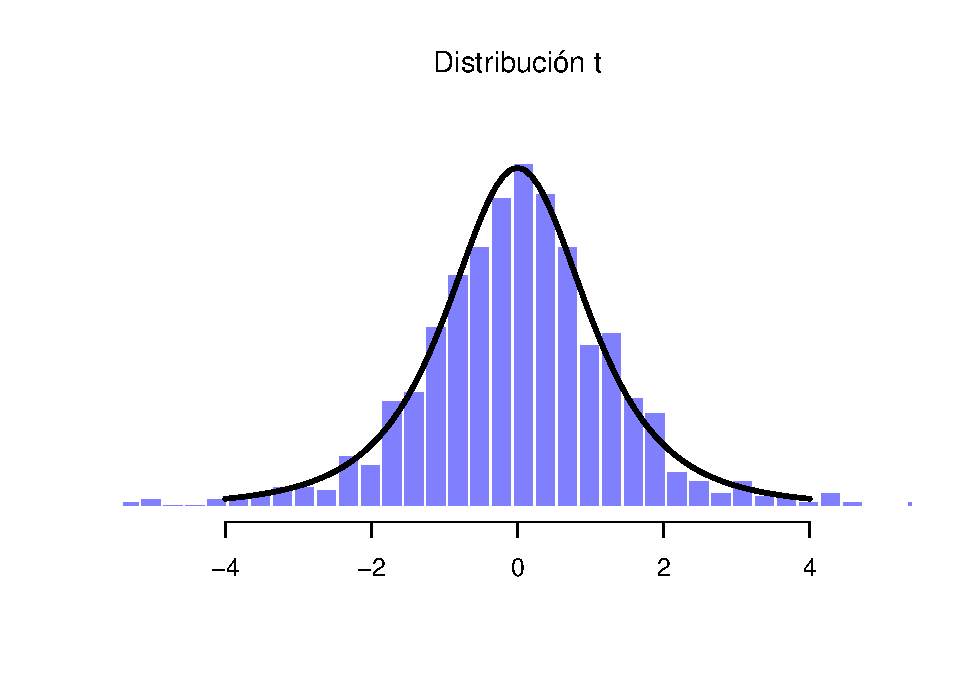
\includegraphics{FdI2_files/figure-latex/distt-1.pdf}
\caption{\label{fig:distt}Distribución t. Es el resultado de dividir una
distribución normal (en este caso la Muestra D) entre una variable
chi-cuadrada escalada}
\end{figure}

Del mismo modo, podemos obtener una distribución \(F\) al dividir dos
distribuciones chi-cuadrada ``escaladas''. Supongamos, por ejemplo, que
deseamos generar datos que sigan una distribución \(F\) con 3 y 20
grados de libertad (es decir, con 3 y 20 variables respectivamente). La
división de los valores de ambas distribuciones nos da como resultado
una nueva variable \texttt{F.3.20} y su distribución es la que se
muestra en la Figura \ref{fig:distf}.

\begin{figure}
\centering
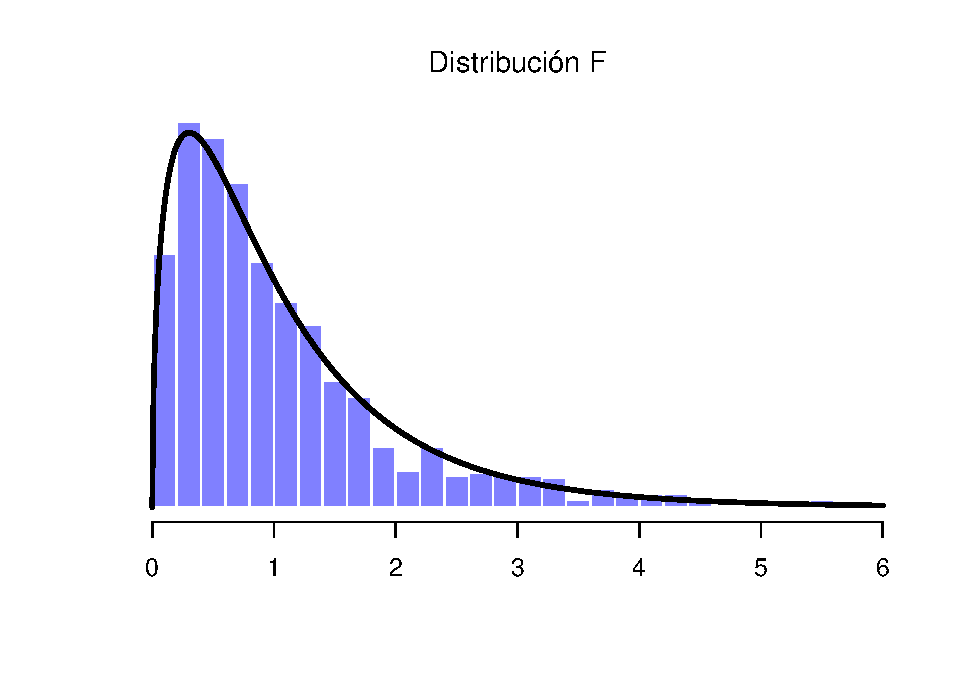
\includegraphics{FdI2_files/figure-latex/distf-1.pdf}
\caption{\label{fig:distf}Distribución F. En este ejemplo hipotético, se
compara la distribución chi-cuadrada de 3 grados de libertad previa con
otra distribución chi-cuadrada con 20 grados de libertad (es decir, que
incluye 20 muestras o variables)}
\end{figure}

Hemos visto tres nuevas distribuciones: \(\chi^2\), \(t\) y \(F\). Todas
son distribuciones continuas, y todas están estrechamente relacionadas
con la distribución normal. Hemos hablado un poco poco sobre la
naturaleza de esta relación. Sin embargo, la clave no es que tengas una
comprensión profunda y detallada de todas estas diferentes
distribuciones, ni que recuerdes las relaciones precisas que existen
entre ellas. Lo más importante es entender la idea básica de que estas
distribuciones están profundamente relacionadas entre sí y a su vez con
la distribución normal. Más adelante en el curso nos vamos a encontrar
con datos que se distribuyen normalmente, o que al menos suponemos que
se distribuyen normalmente. Por lo tanto, si suponemos que nuestros
datos se distribuyen normalmente, debemos saber reconocer las
distribuciones \(\chi^2\), \(t\) y \(F\)..

\section{Resumen}\label{resumen}

En este capítulo hemos hablado de probabilidad. Hemos hablado de lo que
significa la probabilidad y por qué los estadísticos no están muy de
acuerdo en lo que significa. Hablamos sobre las reglas que las
probabilidades tienen que obedecer. Hemos introducido la idea de una
distribución de probabilidad y conocido algunas de las distribuciones de
probabilidad más importantes con las que nos podemos encontrar. Los
temas han sido los siguientes:

\begin{itemize}
\tightlist
\item
  Teoría de probabilidad vs estadística (Sección \ref{probstats})
\item
  Visión frecuenciantista vs visión bayesiana de probabilidad (Sección
  \ref{probmeaning})
\item
  Conceptos básicos de la teoría de probabilidad (Sección
  \ref{basicprobability})
\item
  Distribución binomial (Sección \ref{binomial}), distribución normal
  (sección \ref{normal}), y otras distribuciones (Sección
  \ref{otherdists})
\end{itemize}

Esto es una simple introducción dentro de un gran tema. La teoría de la
probabilidad es una rama de las matemáticas, completamente separada de
su aplicación a la estadística y al análisis de datos. Como tales, hay
miles de libros escritos sobre el tema y las universidades generalmente
ofrecen clases dedicadas por completo a la teoría de la probabilidad. En
este capítulo se han descrito cinco distribuciones de probabilidad
estándar, pero existen \emph{muchas} más que esas. Afortunadamente,
estas distribuciones bastarán por el momento.

Los conceptos básicos que hemos adquirido en este capítulo servirán como
fundamento para los siguientes dos. Existen muchas reglas sobre lo que
se nos ``permite'' decir cuando hacemos inferencia estadística, y muchas
de ellas pueden parecer arbitrarias. Sin embargo, veremos que comienzan
a tener sentido si tenemos en cuenta estos conceptos básicos que hemos
aprendido.

\chapter{Estimación}\label{estimation}

Al comienzo del capítulo inicial, vimos la distinción que existe entre
la \emph{estadística descriptiva} y la \emph{estadística inferencial}.
El papel de la estadística descriptiva es resumir de manera concisa lo
que \emph{ya sabemos}. Por otro lado, el propósito de la estadística
inferencial es ``aprender lo que no sabemos a partir de lo que
hacemos''. Ahora que tenemos cierto conocimiento sobre la teoría de la
probabilidad, podemos pensar en el problema de la inferencia
estadística. ¿Qué tipo de información nos gustaría conocer o aprender?
¿Y cómo lo aprendemos? Estas son las preguntas que se encuentran en el
corazón de la estadística inferencial y tradicionalmente se dividen en
dos ``grandes ideas'': la estimación y la prueba o contraste de
hipótesis. El objetivo de este capítulo es presentar la primera de estas
grandes ideas, la teoría de la estimación. Pero antes, hablaré sobre la
teoría del muestreo, ya que la teoría de la estimación no tiene sentido
hasta que no se comprende el muestreo. Como consecuencia, este capítulo
se divide en dos partes, las secciones \ref{srs} a \ref{samplesandclt}
se centran en la teoría del muestreo, y las secciones
\ref{pointestimates} y \ref{ci} hacen uso de esa teoría del muestreo
para discutir cómo piensan los estadísticos sobre la estimación.

\section{Muestras, poblaciones y muestreo}\label{srs}

Antes hemos hablado sobre el proceso de inducción inferencial, donde
recalcamos que \emph{todo} aprendizaje (o aquello que queremos llegar a
conocer) requiere que hagamos suposiciones. Aceptando que esto es
cierto, hemos de aceptar algunas suposiciones generales sobre los datos
que hemos adquirido para poder utilizarlos. Aquí es donde entra en juego
la \textbf{\emph{teoría del muestreo}}. Si la teoría de la probabilidad
representa los cimientos sobre los que se construye toda la teoría
estadística, la teoría del muestreo es el marco alrededor del cual se
puede construir el resto de la casa. La teoría del muestreo juega un
papel muy importante en la especificación de los supuestos en los que se
basan sus inferencias estadísticas. Y para hablar sobre ``hacer
inferencias'' de la forma en que los estadísticos lo piensan, debemos
ser un poco más explícitos acerca de \emph{qué} es lo que estamos
extrayendo (la muestra) y \emph{sobre qué} es de lo que estamos haciendo
inferencias (la población).

En casi todas las situaciones de interés, lo que tenemos a nuestra
disposición como investigadores es una \emph{muestra} de datos.
Podríamos, por ejemplo, haber realizado un experimento con un cierto
número de participantes; una empresa de encuestas podría haber
telefoneado a algunas personas para hacer preguntas sobre las
intenciones de voto, etc. Independientemente de cual sea el caso, el
conjunto de datos disponibles que tengamos es finito e incompleto. No
podemos conseguir que todas las personas del mundo realicen nuestro
experimento; una empresa de encuestas no tiene el tiempo ni el dinero
para llamar a todos los votantes del país, etc. Para la estadística
descriptiva esta muestra es lo único que importa. Con la estadística
inferencial daremos un paso más allá.

\subsection{Definición de una población}\label{pop}

Una muestra es una cosa muy concreta. Puedes abrir un archivo de Excel y
ahí podrás encontrar los datos de una muestra. Una
\textbf{\emph{población}}, por otro lado, es una idea más abstracta. Se
refiere al conjunto de todas las personas posibles, o todas las
observaciones posibles, sobre las que desea sacar conclusiones y, en
general, es \emph{mucho} más grande que la muestra. En un mundo ideal,
el investigador comenzaría el estudio con una idea clara de cuál es la
población de interés, ya que el proceso de diseñar un estudio y probar
una hipótesis sobre los datos que produce depende de la población sobre
la que se quiere hacer afirmaciones. Sin embargo, en la práctica esto no
sucede siempre: por lo general, el investigador tiene una idea bastante
vaga de lo que es la población y diseña el estudio lo mejor que puede
sobre esa base.

A veces es fácil indicar cuál es la población de interés. En el ejemplo
de la ``empresa de encuestas'' que vimos en el capítulo anterior, la
población consistía en todos los votantes inscritos en un momento del
estudio: varios millones de personas. En cambio, la muestra fue un
conjunto de 1,000 personas que pertenecen todas a esa población. Sin
embargo, en la mayoría de los casos, definir esta muestra/población no
es tan fácil. En estudios o experimentos con seres humanos, determinar
la población de interés es un poco más complicado. Supongamos que
realizo un experimento con 100 estudiantes de pregrado que representan
mi muestra. Mi objetivo es, por ejemplo, intentar aprender algo sobre
cómo una intervención educativa modifica la dinámica de una clase.
Tomando en cuento a la muestra que tenemos, ¿cuál de las siguientes
opciones contará como ``la población''?:

\begin{itemize}
\tightlist
\item
  ¿Todos los estudiantes de educación de la Universidad de Navarra?\\
\item
  ¿Estudiantes de grado en educación en general, de cualquier parte del
  mundo?\\
\item
  ¿Españoles vivos actualmente?\\
\item
  ¿Españoles de edades similares a las de mi muestra?
\item
  ¿Hispanoparlantes?
\item
  ¿Cualquier persona viva actualmente?\\
\item
  ¿Cualquier ser humano, pasado, presente o futuro?
\end{itemize}

Cada una de estas opciones define un grupo real de personas, las cuales
podrían ser todas de interés para mí como investigador en educación, y
no es tan obvio cuál debería ser la verdadera población de interés.

\subsection{Muestras aleatorias
simples}\label{muestras-aleatorias-simples}

\begin{figure}
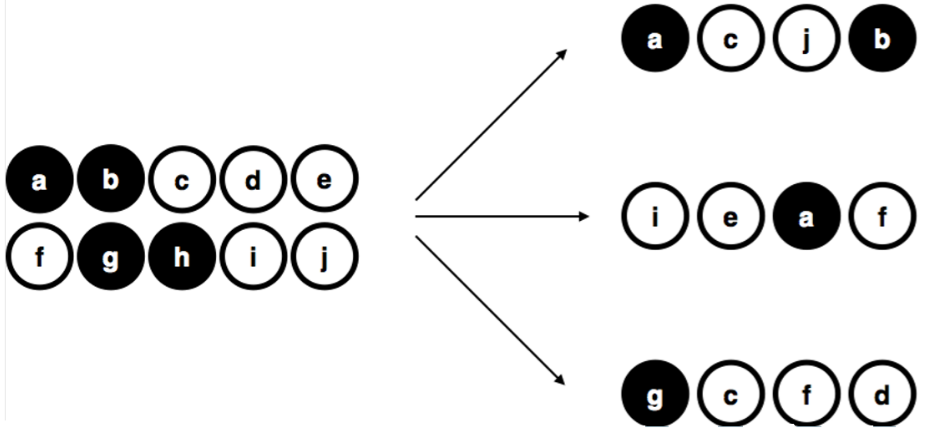
\includegraphics[width=12.86in]{img/estimation/srs1} \caption{Muestreo aleatorio simple *sin* reemplazo de una población finita.}\label{fig:srs1}
\end{figure}

Independientemente de cómo definamos a una población, la clave es que la
muestra es un subgrupo de esa población, y nuestro objetivo es utilizar
nuestro conocimiento de la muestra para hacer inferencias sobre las
propiedades de la población. La relación que exista entre los dos
dependerá del \emph{procedimiento} mediante el cual se seleccionó la
muestra. Este procedimiento se conoce como \textbf{\emph{método de
muestreo}} y es importante comprender su importancia.

Pongamos un ejemplo sencillo. Imaginemos que tenemos una bolsa que
contiene 10 fichas. Cada ficha tiene una letra única impresa, con la que
la podemos distinguir de entre las otras 10 fichas. Las fichas vienen en
dos colores, blanco y negro. Este conjunto de fichas es la población de
interés y se muestra gráficamente a la izquierda de la Figura
\ref{fig:srs1}. Como podrás ver en la imagen, tenemos 4 fichas negras y
6 fichas blancas, pero recuerda que en la vida real esto no lo sabríamos
a menos que miráramos en la bolsa. Ahora imagina que realizas el
siguiente ``experimento'': agitas la bolsa, cierras los ojos y sacas 4
fichas sin devolver ninguna de ellas a la bolsa. Primero sale la ficha
\(a\) (negra), seguida de la ficha \(c\) (blanca), luego la \(j\)
(blanca) y finalmente la ficha \(b\) (negra). Una vez extraídas 4
fichas, podrás volver a poner todas las fichas en la bolsa y repetir el
experimento, como se muestra en el lado derecho de la Figura
\ref{fig:srs1}. Cada vez que repites el experimento obtienes resultados
diferentes, pero el procedimiento es idéntico en cada caso. El hecho de
que el mismo procedimiento pueda dar lugar a resultados diferentes cada
vez, lo define como un proceso \emph{aleatorio}. Y debido a que hemos
agitado la bolsa antes de sacar las fichas, parece razonable pensar que
todas las fichas tienen las mismas posibilidades de ser seleccionadas.
Un procedimiento en el que todos los miembros de la población tienen las
mismas posibilidades de ser seleccionados se denomina
\textbf{\emph{muestra aleatoria simple}}. El hecho de que se \emph{no}
se devuelvan las fichas a la bolsa después de salir, significa que no
podremos observar la misma ficha dos veces, y en tales casos se dice que
ha habido un muestreo \textbf{\emph{sin reemplazo}}.

Para comprender la importancia del procedimiento de muestreo,
consideremos ahora una forma alternativa en la que podría haberse
realizado el experimento. Supongamos que mi sobrino de 3 años coge la
bolsa y decide sacar las cuatro fichas negras (le gusta el color negro)
sin devolverlas la bolsa. Este esquema de muestreo \emph{sesgado} se
muestra en la Figura \ref{fig:brs}. Ahora considera el valor que tiene
obtener una muestra con 4 fichas negras y 0 fichas blancas siguiendo el
procedimiento de mi sobrino. Vemos pues, como el valor dependerá mucho
del método de muestreo. Si sabemos que el método de muestreo está
sesgado para seleccionar únicamente fichas negras, entonces una muestra
que consta únicamente de fichas negras no dice mucho sobre nuestra
población de fichas. Por esta razón, los estadísticos prefieren que un
conjunto de datos provenga de una muestra aleatoria simple, ya que
facilita \emph{mucho} el análisis de los datos.

\begin{figure}
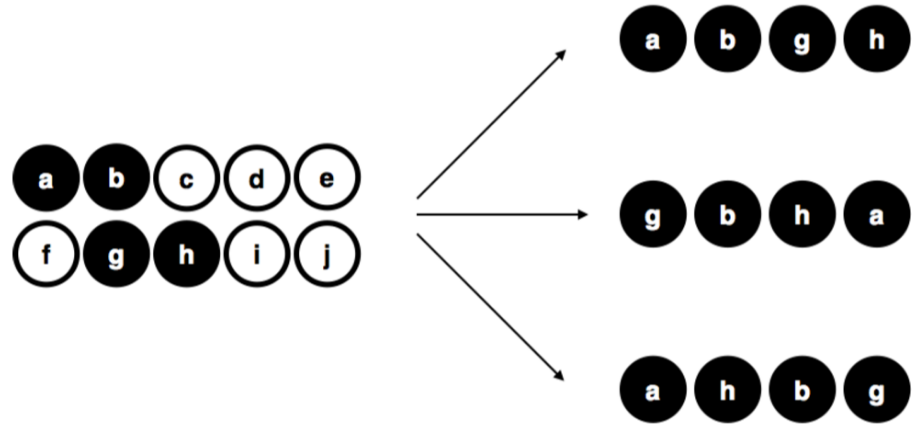
\includegraphics[width=12.81in]{img/estimation/brs} \caption{Muestreo sesgado sin reemplazo de una población finita.}\label{fig:brs}
\end{figure}

\begin{figure}
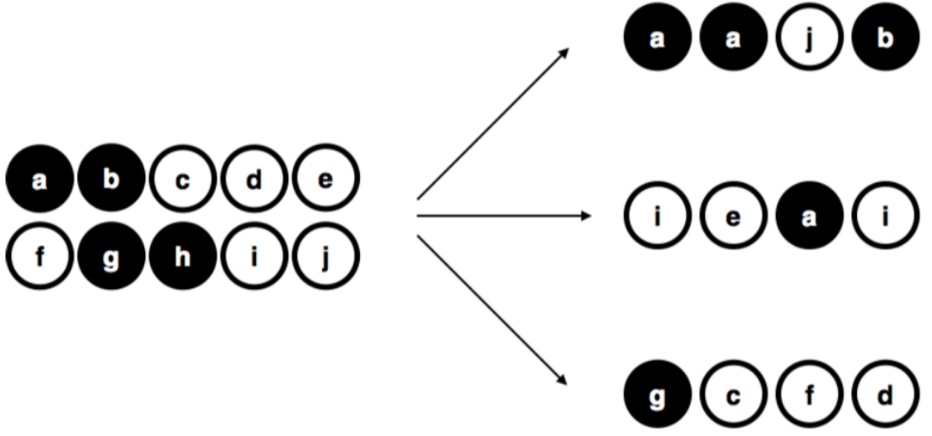
\includegraphics[width=12.94in]{img/estimation/srs2} \caption{Muestreo aleatorio simple *con* reemplazo de una población finita.}\label{fig:srs2}
\end{figure}

Vale la pena mencionar un tercer procedimiento. Esta vez cerramos los
ojos, agitamos la bolsa y sacamos una ficha. Sin embargo, esta vez
registramos la observación y luego volvemos a poner la ficha dentro de
la bolsa. Nuevamente, cerramos los ojos, agitamos la bolsa y sacamos
otra ficha. Repetimos este procedimiento hasta que tengamos 4 fichas.
Los conjuntos de datos que hemos generado de esta manera siguen siendo
muestras aleatorias simples, pero debido a que volvemos a meter las
fichas dentro de la bolsa inmediatamente después de haberlas sacado, se
denomina como una muestra \textbf{\emph{con reemplazo}}. La diferencia
entre este caso y el primero es que es posible observar al mismo
elemento de la población varias veces (en este caso la misma ficha), tal
como se ilustra en la Figura \ref{fig:srs2}.

Por lo general, la mayoría de los experimentos que veamos en ciencias de
la educación tienden a tomar muestras sin reemplazo, ya que la misma
persona no puede participar en el experimento dos veces. Sin embargo,
una gran parte de la teoría estadística se basa en el supuesto de que
los datos surgen de una muestra aleatoria simple \emph{con} reemplazo.
En la vida real, esto rara vez importa. Si la población de interés es
grande, la diferencia entre el muestreo con y sin reemplazo es demasiado
pequeña como para preocuparnos. Sin embargo, la diferencia que existe
entre muestras aleatorias simples y muestras sesgadas no es algo no es
algo que podemos ignorar tan facilmente.

\subsection{La mayoría de las muestras no son muestras aleatorias
simples}\label{la-mayoria-de-las-muestras-no-son-muestras-aleatorias-simples}

Si miras la lista anterior de posibles poblaciones, te darás cuenta que
es casi imposible obtener una muestra aleatoria simple de la mayoría de
esas poblaciones de interés. Cuando hacemos experimentos con estudiantes
universitarios, el obtener una verdadera muestra aleatoria de estos
estudiantes los podemos considerar como un milagro menor, aunque al
final se trate de una población muy específica a partir de la cual
generalizar. Mencionaré brevemente algunos de los otros tipos de
muestreo que existen y que solemos encontrar con frecuencia:

\begin{itemize}
\item
  \emph{Muestreo estratificado}. Supongamos que tu población está (o
  puede estar) dividida en varias subpoblaciones o \emph{estratos}
  diferentes. Quizás sea porque estás realizando un estudio en varios
  paises diferentes, por ejemplo. En lugar de intentar tomar una muestra
  aleatoria de toda la población en su conjunto, recolectamos una
  muestra aleatoria de cada una de las subpoblaciones o estratos. El
  muestreo estratificado suele ser más fácil de llevar a cabo que el
  muestreo aleatorio simple, especialmente cuando la población ya está
  dividida en los distintos estratos. También puede ser más eficiente
  que el muestreo aleatorio simple, especialmente cuando algunas de las
  subpoblaciones son raras o poco frecuentes. Por ejemplo, en el estudio
  de la esquizofrenia, resulta más sencillo dividir la población en dos
  estratos (con-esquizofrenia y sin-esquizofrenia) y adquirir una
  muestra de cada grupo. Si seleccionaramos personas al azar,
  obtendríamos tan pocas personas con esquizofrenia en la muestra que el
  estudio resultaría inútil.
\item
  \emph{Muestreo de bola de nieve}. Es una técnica que es especialmente
  útil cuando se toman muestras de una población ``oculta'' o de difícil
  acceso, y es especialmente común en las ciencias sociales. Por
  ejemplo, supongamos que los investigadores quieren realizar una
  encuesta de opinión a personas VIH positivo. Es posible que el equipo
  de investigación solo tenga los datos de contacto de algunas personas
  VIH positivo, por lo que la encuesta comienza pidiéndoles a esas
  personas que participen (etapa 1). Al final de la encuesta, se pide a
  los participantes que proporcionen los datos de contacto de otras
  personas que podrían querer participar. En la etapa 2, se encuesta a
  estos nuevos contactos. El proceso continúa hasta que los
  investigadores obtengan datos suficientes. La gran ventaja del
  muestreo de bola de nieve es que es capaz de proporcionar datos en
  situaciones que de otro modo serían imposibles de obtener. Desde el
  punto de vista estadístico, la principal desventaja es que la muestra
  es altamente no aleatoria y no aleatoria en formas que son difíciles
  de abordar.
\item
  \emph{Muestreo de conveniencia}. En este tipo de muestreo las muestras
  se eligen de una forma conveniente para el investigador, sin que
  exista una selección al azar a partir de la población de interés. El
  muestreo de bola de nieve es un tipo de muestreo de conveniencia, pero
  hay muchos otros. Un ejemplo son los estudios que se basan en
  estudiantes de universitarios. Estas muestras generalmente no son
  aleatorias desde dos puntos de vista: en primer lugar, depender de una
  muestra de estudiantes universitarios significa automáticamente que
  estos datos están restringidos a una sola subpoblación. En segundo
  lugar, los estudiantes suelen elegir los estudios en los que
  participan, por lo que la muestra es un subconjunto de estudiantes
  autoseleccionado, no un subconjunto seleccionado al azar. En general,
  la mayoría de los estudios incluyen muestras de conveniencia de una
  forma u otra. A veces, puede suponer una limitación en la
  interpretación de los resultados, pero no siempre.
\end{itemize}

\subsection{¿Cuánto importa si no se tiene una muestra aleatoria
simple?}\label{cuanto-importa-si-no-se-tiene-una-muestra-aleatoria-simple}

Hemos visto que en muchos casos no es posible recolectar muestras
aleatorias simples. ¿Eso qué impacto tiene? Un ejemplo de ese impacto lo
podemos apreciar con la diferencia que existe entre las Figuras
\ref{fig:srs1} y \ref{fig:brs}. Sin embargo, no es tan malo como parece.
Algunos tipos de muestras sesgadas no representan ningún problema. Por
ejemplo, cuando utilizamos el muestreo estratificado, realmente sabemos
\emph{cuál} es el sesgo ya que lo hemos creado deliberadamente, con la
intención de \emph{aumentar} la efectividad de su estudio, y existen
técnicas estadísticas que podemos utilizar para ajustar estos sesgos que
hemos introducido. En estos casos, por lo tanto, no tenemos un problema.

Sin embargo, es importante recordar que el muestreo aleatorio es un
medio para un fin, no el fin en sí mismo. Supongamos que recolectamos
una muestra de conveniencia y, como tal, podemos asumir que está
sesgada. Un sesgo en el método de muestreo solo es un problema si nos
hace sacar conclusiones equivocadas. Desde esta perspectiva, podemos
afirmar que no necesitamos que la muestra sea aleatoria en \emph{todos}
los aspectos: necesitamos que sea aleatoria con respecto al fenómeno de
interés que buscamos estudiar. Supongamos que estoy haciendo un estudio
sobre la capacidad de atención sostenida en niños de 6 años. En el
estudio 1, tengo la capacidad de tomar muestras al azar de todos los
niños de 6 años del mundo actualmente vivos, con una pequeña excepción:
sólo puedo incluir niños nacidos en lunes. En el estudio 2, puedo tomar
una muestra al azar de la población española. Con estos estudios quiero
generalizar mis resultados a la población de todos los niños de 6 años.
¿Qué estudio es mejor? La respuesta, obviamente, es el estudio 1. ¿Por
qué? Porque no tenemos ninguna razón para pensar que ``nacer en lunes''
influye en la capacidad de atención sostenida. Por otro lado, puedo
pensar en varias razones por las que ``ser español'' podría ser
importante. España es un país rico e industrializado con un sistema
educativo muy desarrollado. Las personas que crecieron con este sistema
habrán tenido experiencias de vida mucho más similares a las
experiencias de vida de las personas que diseñaron las pruebas de
capacidad de atención sostenida. Esta experiencia compartida podría
traducirse fácilmente en creencias similares sobre cómo se debe
``realizar una prueba'', entre otras razones. Este tipo de
características son importantes y podrían, por ejemplo, llevar a una
imagen engañosa de lo que es la capacidad atención sostenida.

Existe un reflexión clave oculta en esta discusión. Al diseñar estudios,
es importante pensar en la población de interés y en esforzarse por
elegir un método de muestreo que sea apropiado para esa población. En la
práctica, muchas veces nos veremos obligados a utilizar una ``muestra de
conveniencia'' (por ejemplo, estudiantes de unos pocos centros), pero
deberíamos, al menos, dedicar un tiempo a pensar en los riesgos e
implicaciones de esta práctica.

\subsection{Parámetros poblacionales y estadísticos
muestrales}\label{parametros-poblacionales-y-estadisticos-muestrales}

Hasta ahora hemos estado hablando de poblaciones como lo haría un
científico. Para un educador, una población puede ser un grupo de niños.
Para un ecologista, una población puede ser un grupo de osos. En la
mayoría de los casos, las poblaciones son cosas concretas que realmente
existen en el mundo real. Los estadísticos, sin embargo, tienen un
interés dual. Por un lado, \emph{están} interesados en los datos del
mundo real de la misma forma que los científicos. Por otro lado, también
operan en el ámbito de la abstracción pura como lo hacen los
matemáticos. En consecuencia, la teoría estadística puede ser un poco
abstracta cuando define una población. Para ello, los estadísticos
operacionalizan el concepto de ``población'' en términos de objetos
matemáticos los cuales ya conocemos: se llaman distribuciones de
probabilidad.

La idea es muy simple. Digamos que estamos hablando (otra vez) de
puntajes de coeficiente intelectual (CI). Para un educador, la población
de interés es un grupo de humanos reales que tienen puntajes de CI. Un
estadístico ``simplifica'' esto al definir operativamente a la población
como la distribución de probabilidad representada en la Figura
\ref{fig:IQdista}. Las pruebas de CI están \emph{diseñadas} de tal forma
que la media sea 100, que la desviación estándar sea 15 y que la
distribución de los puntajes sea normal. Estos valores se denominan
\textbf{\emph{parámetros poblacionales}} porque son característicos de
toda la población. Es decir, decimos que la media de la población
\(\mu\) es 100, y la desviación estándar de la población \(\sigma\) es
15.

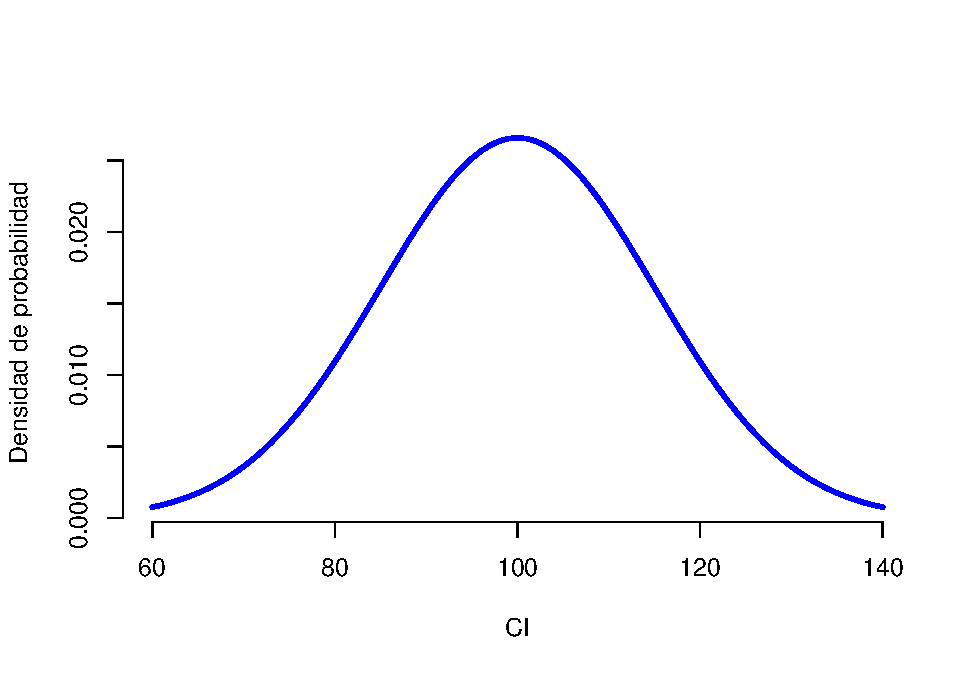
\includegraphics{FdI2_files/figure-latex/IQdista-1.pdf}
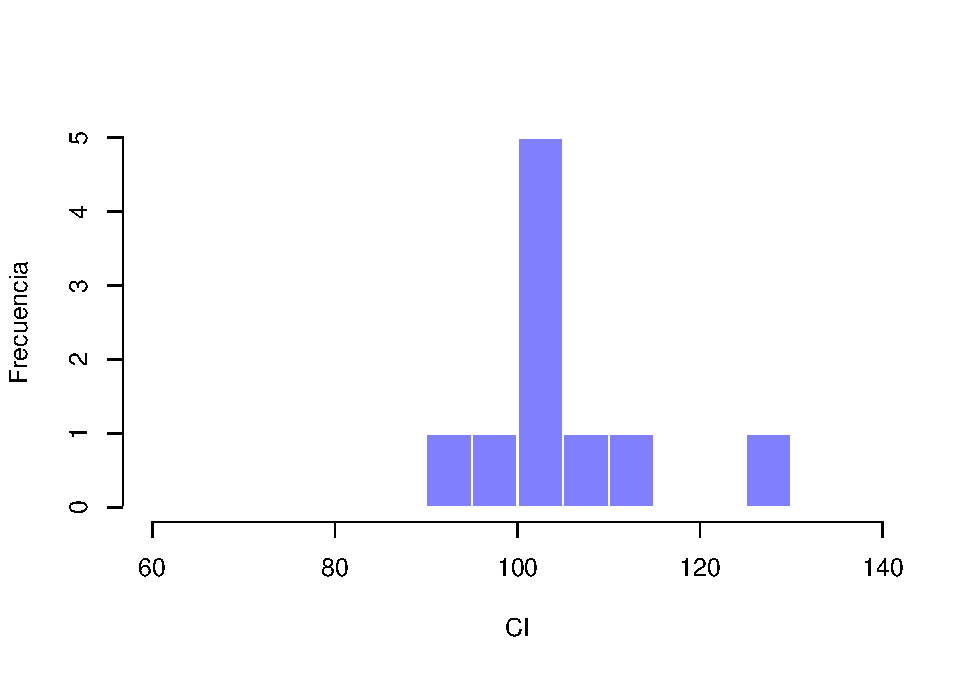
\includegraphics{FdI2_files/figure-latex/IQdistb-1.pdf}

\begin{verbatim}
## [1] "n= 10 mean= 105.604149145068 sd= 9.38271457854891"
\end{verbatim}

Supongamos que hacemos un experimento. Seleccionamos 100 personas al
azar para que elaboren nuestro test de CI, lo cual me dará una muestra
aleatoria de la población. Mi muestra consistirá en una serie de números
como estos:

\begin{verbatim}
                          106 101 98 80 74 ... 107 72 100
\end{verbatim}

Estos puntajes forman parte de una muestra extraída de una población con
distribución normal, media de 100 y desviación estándar de 15. Si
trazamos un histograma de esta muestra, obtendremos algo como el que se
muestra en la Figura \ref{fig:IQdistb}. Podemos ver que el histograma
tiene una forma \emph{aproximadamente} normal, pero aún queda como una
aproximación burda de la verdadera distribución de la población que se
muestra en la Figura \ref{fig:IQdista}. Si calculamos la media muestral,
obtendremos un número que está bastante cerca de la media de la
población 100, pero no es idéntico. En este caso, vemos que las personas
de mi muestra tienen un CI medio de 98,5 y la desviación estándar de sus
puntuaciones de CI es de 15,9. Estos \textbf{\emph{estadísticos
muestrales}} nos presentan una descripción de nuestro conjunto de datos
y, aunque son bastante similares a los valores reales de población, no
son iguales. En general, los estadísticos muestrales son lo que podemos
calcular a partir de un conjunto de datos mientras que los parámetros
poblacionales son las cosas sobre las que deseamos aprender. Más
adelante, hablaremos sobre cómo podemos estimar los parámetros
poblacionales utilizando sus estadísticos muestrales (Sección
\ref{pointestimates}) así como qué tan seguros estamos de esos
estimadores (Sección \ref{ci}) pero antes necesitamos conocer algunos
conceptos adicionales sobre la teoría de muestreo.

\section{La ley de los grandes números}\label{lawlargenumbers}

En la sección anterior vimos los resultados de un experimento ficticio
con un tamaño de muestra de \(N=100\). Los resultados fueron algo
alentadores: la media real de la población es 100,,mientras que la media
muestral fue de 98.5, una aproximación razonable. En muchos estudios
científicos, este nivel de precisión es perfectamente aceptable, pero
existen situaciones en las que nos gustaría ser bastante más precisos.
Si queremos que nuestros estadísticos muestrales se acerquen más a los
parámetros poblacionales, ¿qué podemos hacer al respecto?

La respuesta lógica sería recolectar más datos. Supongamos que hacemos
un experimento más grande, en el cual medimos el CI de 10,000 personas.
Si entrás \href{https://leudave.shinyapps.io/sampling/}{aquí} podrás
hacer una simulación. El histograma de esta simulación se muestra en la
Figura \ref{fig:IQdistc}. Una inspección rápida nos revelará que una
muestra de mayor tamaño representa una mejor aproximación a la
distribución poblacional real, especialmente si la comparamos con la
muestra más pequeña. Esto también se ve reflejado en los estadísticos
muestrales: el CI medio de la muestra grande es de 99.9 y su desviación
estándar es de 15.1. Estos valores son muy cercanos a los valores reales
de la población.

\begin{figure}
\centering
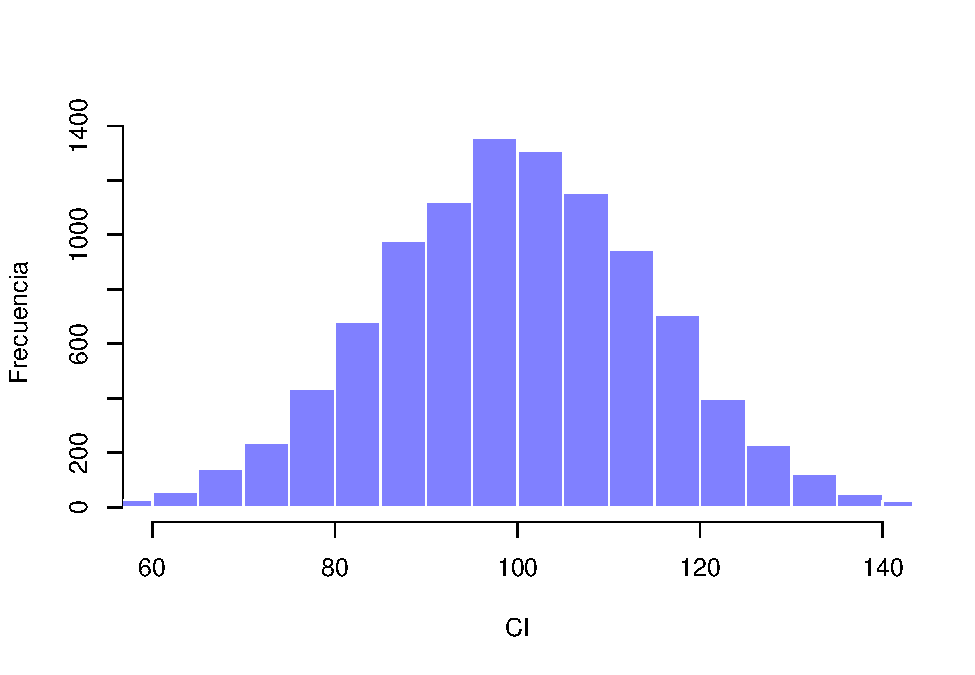
\includegraphics{FdI2_files/figure-latex/IQdistc-1.pdf}
\caption{\label{fig:IQdistc}Muestra con 10,000 observaciones provenientes de
la distribución poblacional previa.}
\end{figure}

Con esto, podemos observar algo que parece obvio: entre más datos
tengamos, mejores resultados obtendremos. Esta intuición tan evidente
que compartimos todos, los estadísticos la definen como la
\textbf{\emph{ley de los grandes números}}. La ley de los grandes
números es una ley matemática que aplica a muchos estadísticos
muestrales, pero la forma más sencilla de entenderla es a través de la
ley aplicada a las medias. Cuando se aplica a la media muestral, la ley
de los grande números nos dice que conforme aumenta el tamaño de
muestra, el valor de la media muestral se acercará al valor de la media
poblacional real. O, para ser más precisos, conforme el tamaño muestral
se aproxima al infinito (escrito como \(N \rightarrow \infty\)) la media
nuestral se aproximará a la media poblacional
(\(\bar{X} \rightarrow \mu\)).\footnote{Técnicamente, la de ley de los
  grandes números es aplicable a cualquier estadístico muestral que
  pueda ser descrito como un promedio de cantidades independiente. La
  varianza muestral, por ejemplo, puede ser representado como un tipo de
  promedio y por ello, sujeto a la ley de los grandes números. Sin
  embargo, el valor mínimo muestral no puede ser interpretado como un
  promedio de nada, y por tanto, no es gobernado por la ley de los
  grandes números.}

Espero que quede patente la importancia de la ley de los grandes números
como una herramienta elemental en la teoría estadística. Esta ley de los
grandes números es nuestro argumento para justificar nuestra creencia de
que recolectar cada vez más y más datos nos acercará a la verdad. Para
cualquier conjunto de datos, los estadísticos muestrales que calculemos
estarán equivocados, pero la ley de los grandes números nos dice que si
seguimos recolectando datos esos estadísticos muestrales tenderán a a
acerca más y más a los parámetros poblacionales reales.

\section{Distribuciones muestrales y el teorema del límite
central}\label{samplesandclt}

La ley de los grandes números es una herramienta muy poderosa, pero no
será suficiente para responder a todas nuestras preguntas. Entre otras
cosas, lo que nos da esta ley es una ``garantía a largo plazo''. A largo
plazo, si pudiéramos recolectar una cantidad infinita de datos, la ley
de los grandes números nos garantiza que los estadísticos muestrales
serán correctos.

Sin embargo, esta ``garantía a largo plazo'' es de poca utilidad en la
vida real: no basta con decir que \emph{con el tiempo} llegaremos a la
respuesta correcta cuando calculemos la media muestral. Saber que un
conjunto de datos infinitamente largo me dará el valor exacto de la
media poblacional es inconciliable con el \emph{hecho} de que mi
conjunto de datos tiene un tamaño de muestra de \(N=100\). En la vida
real, tenemos que saber algo más sobre el comportamiento de la media
muestral de una muestra modesta como la nuestra.

\subsection{Distribución muestral de la media}\label{samplingdists}

Abandonemos por un momento la idea de tener tamaños de muestra de 10,000
y pensemos en un experimento más modesto. Esta vez extraemos una muestra
de \(N=5\) personas y medimos su CI. Este es el resultado:

\begin{verbatim}
90  82  94  99 110
\end{verbatim}

El CI medio de esta muestra es exactamente 95. Esta muestra nos revela
un valor mucho menos preciso que en el experimento previo. Ahora imagina
que decides \textbf{\emph{replicar}} este mismo experimento. Es decir,
quieres repetir el mismo procedimiento de tal forma que selecciones una
nueva muestra aleatoria de 5 personas y obtener su CI una vez más. Estos
son los CI de nuestra nueva muestra:

\begin{verbatim}
78  88 111 111 117
\end{verbatim}

Al calcular la media de esta muestra vemos que es de 101. Si repetimos
el experimento 10 veces más obtendremos los resultados que se muestran
en la siguiente Tabla. Con ella podrás ver que la media muestral cambia
con cada replicación del experimento.

\begin{tabular}{l|r|r|r|r|r|r}
\hline
. & P1 & P2 & P3 & P4 & P5 & Media.Muestral\\
\hline
Rep 1 & 90 & 82 & 94 & 99 & 110 & 95.0\\
\hline
Rep 2 & 78 & 88 & 111 & 111 & 117 & 101.0\\
\hline
Rep 3 & 111 & 122 & 91 & 98 & 86 & 101.6\\
\hline
Rep 4 & 98 & 96 & 119 & 99 & 107 & 103.8\\
\hline
Rep 5 & 105 & 113 & 103 & 103 & 98 & 104.4\\
\hline
Rep 6 & 81 & 89 & 93 & 85 & 114 & 92.4\\
\hline
Rep 7 & 100 & 93 & 108 & 98 & 133 & 106.4\\
\hline
Rep 8 & 107 & 100 & 105 & 117 & 85 & 102.8\\
\hline
Rep 9 & 86 & 119 & 108 & 73 & 116 & 100.4\\
\hline
Rep 10 & 95 & 126 & 112 & 120 & 76 & 105.8\\
\hline
\end{tabular}

Supongamos ahora que decidimos continuar con este procedimiento,
replicando el experimento de ``5 puntuaciones de CI'' una y otra vez. Y
cada vez, obtendremos una media muestral diferente, que en el caso de
los 10 experimentos que ya hemos hecho corresponderían con los
siguientes valores:

\begin{verbatim}
                      95.0 101.0 101.6 103.8 104.4 ...
\end{verbatim}

¿Qué pasaría si continuamos y recolectamos 10,000 medias muestrales y
trazamos un histograma con ellas? Obtendríamos un resultado como el que
vemos en la Figura \ref{fig:sampdistmean}. En esta imagen podemos
apreciar que la media muestral de ``5 puntuaciones de CI'' se encuentra,
por lo general, entre 90 y 110. Pero lo más interesante de esta Figura
es que demuestra el hecho de que si repetimos el experimento una y otra
vez, ¡lo que obtenemos es una \emph{distribución} de las medias
muestrales! Esta distribución recibe un nombre especial en estadística:
se le llama \textbf{\emph{distribución muestral de la media}}.

Las distribuciones muestrales son una idea teórica importante en la
estadística, y además, son cruciales si queremos entender cómo se
comportan las muestras pequeñas. Por ejemplo, cuando realizamos el
primer experimento con 5 puntuaciones de CI, la media muestral fue de
95. Sin embargo, lo que la distribución muestral nos dice en la Figura
\ref{fig:sampdistmean}, es que este experimento con 5 puntuaciones no es
muy preciso. Si repetimos el experimento muchas veces, la distribución
muestral nos dice que podemos esperar que la media muestral esté entre
80 y 120.

\begin{figure}
\centering
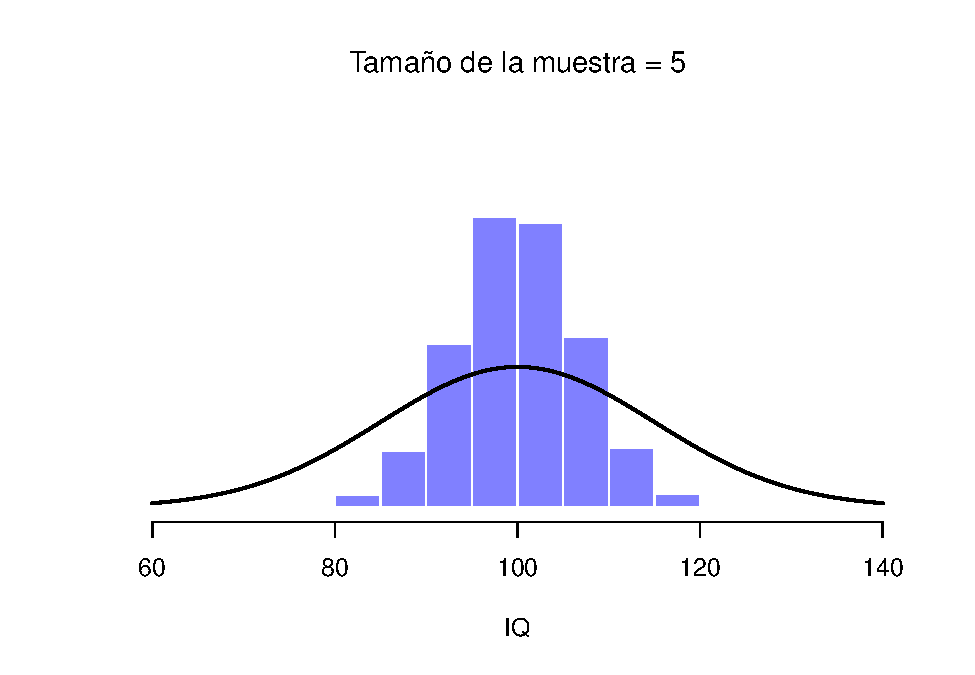
\includegraphics{FdI2_files/figure-latex/sampdistmean-1.pdf}
\caption{\label{fig:sampdistmean}La distribución muestral de la media en el
experimento con 5 puntuaciones de CI. Si obtenemos una muestra aleatoria
de 5 personas y calculamos la \emph{media} de sus puntajes, obtendremos
casi con seguridad un valor entre 80 y 120, aunque existen individuos
que tienen un CI mayor de 120 o menor de 80. La línea negra dibuja la
distribución poblacional de los puntajes de CI para comparar.}
\end{figure}

\subsection{Existen distribuciones muestrales para cualquier estadístico
muestral}\label{existen-distribuciones-muestrales-para-cualquier-estadistico-muestral}

Una cosa que debemos tener en cuenta cuando pensemos sobre las
distribuciones muestrales es que es posible estimarlos a partir de
\emph{cualquier} estadístico muestral. Por ejemplo, supongamos que en
cada una de las veces que replicamos el ``experimento con 5 puntajes de
CI'' también tomamos nota del valor de CI máximo en cada experimento.
Esto daría como resultado una serie de número que empezaría de esta
forma:

\begin{verbatim}
                      110 117 122 119 113 ... 
\end{verbatim}

Si hacemos esto una y otra vez obtendremos una distribución muestral muy
diferente, concretamente la \emph{distribución muestral del valor
máximo}. La distribución muestral del valor máximo de 5 puntajes de CI
se muestra en la Figura \ref{fig:sampdistmax}. No es de sorprender, que
si escogemos a 5 personas al azar y seleccionamos a la persona con el
puntaje más alto, este tenga un CI superior a la media. Y de hecho, la
mayoría de las veces nos encontraremos con puntajes de CI en el rango
entre 100 y 140.

\begin{figure}
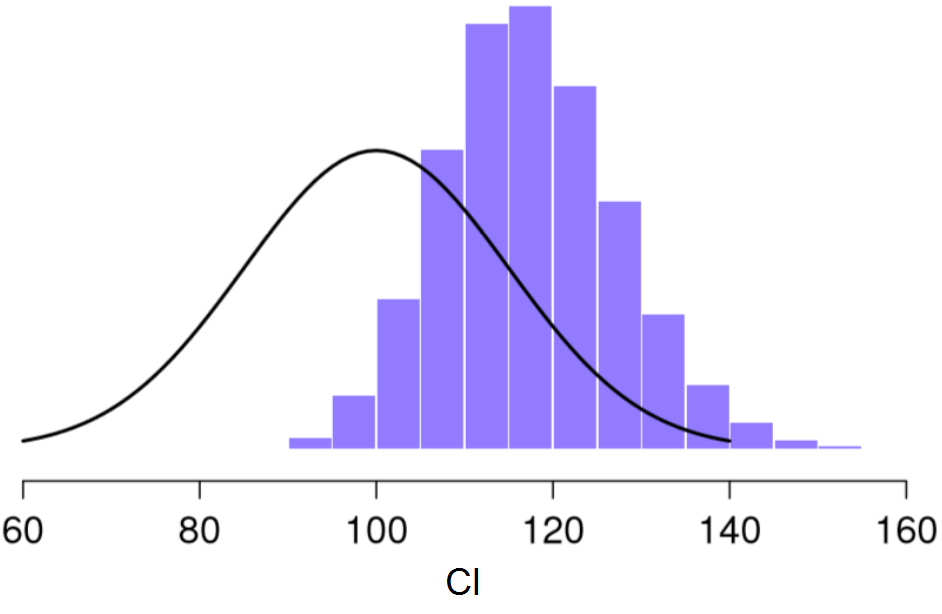
\includegraphics[width=13.08in]{img/estimation/sampdistmax} \caption{Distribución muestral del valor máximo de CI}\label{fig:sampdistmax}
\end{figure}

\subsection{El teorema del límite central}\label{clt}

A continuación verás una serie de ilustraciones en las que podremos
observar como influye el tamaño de la muestra en las distribuciones
muestrales. Estas distribuciones muestrales se han generado a partir
10,000 muestras de datos sobre el CI, donde se ha calculado la media
muestral de cada una de esas muestras. Los histogramas muestran la
distribución de esas medias muestrales (en otras palabras, son
distribuciones muestrales de la media). Cada valor individual de CI fue
extraído de una distribución normal con media de 100 y desviación
estándar de 15, que se muestra como una línea sólida de color negro.

\begin{figure}
\centering
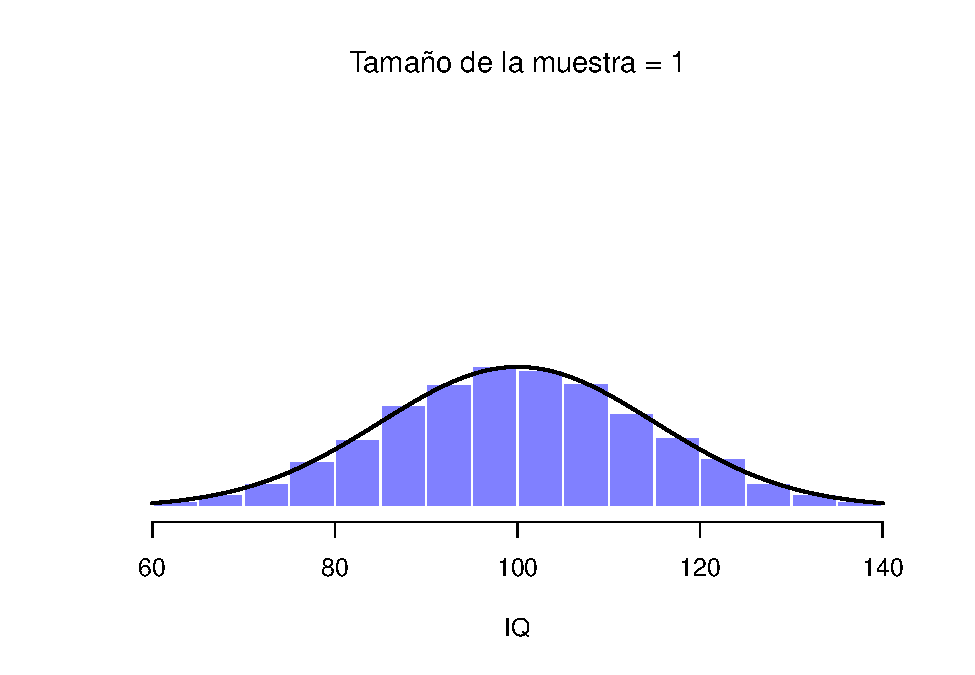
\includegraphics{FdI2_files/figure-latex/IQsampa-1.pdf}
\caption{\label{fig:IQsampa}Esta distribución muestral parte de una sola
observación (tamaño muestral de 1), de forma que la media muestral es el
puntaje de CI de una persona. Como consecuencia, la distribución
muestral de la media es idéntica a la distribución poblacional de los
valores de CI.}
\end{figure}

\begin{figure}
\centering
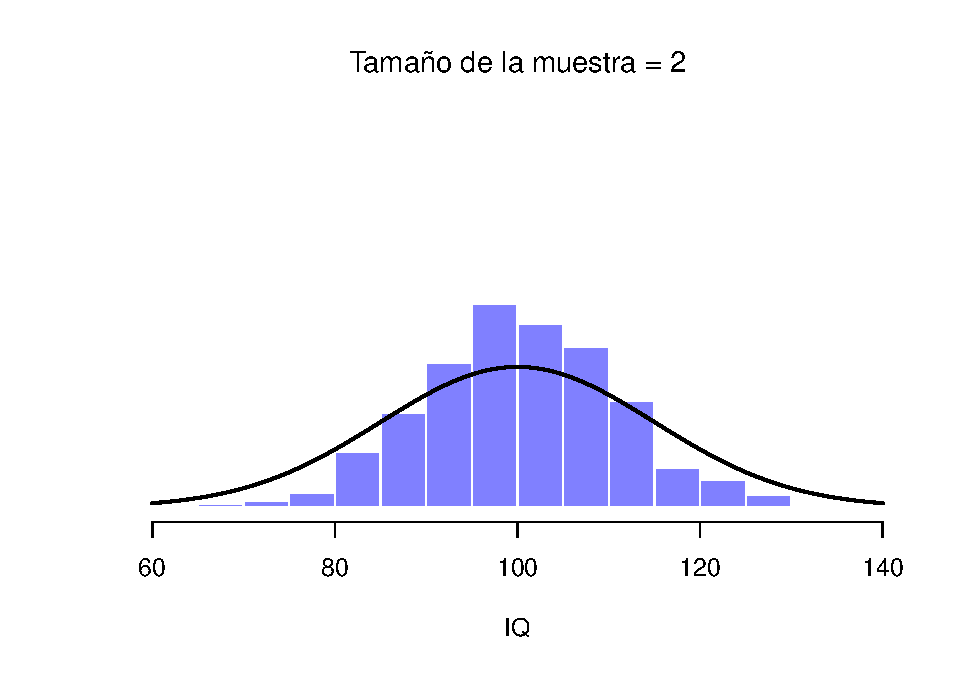
\includegraphics{FdI2_files/figure-latex/IQsampb-1.pdf}
\caption{\label{fig:IQsampb}Cuando aumentamos el tamaño de la muestra a 2,
la media de cualquier muestra tiende a acercarse más a la media
poblacional que a un puntaje individual de CI, por lo que el histograma
(distribución muestral) es un poco más estrecho que el de la
distribución de la población.}
\end{figure}

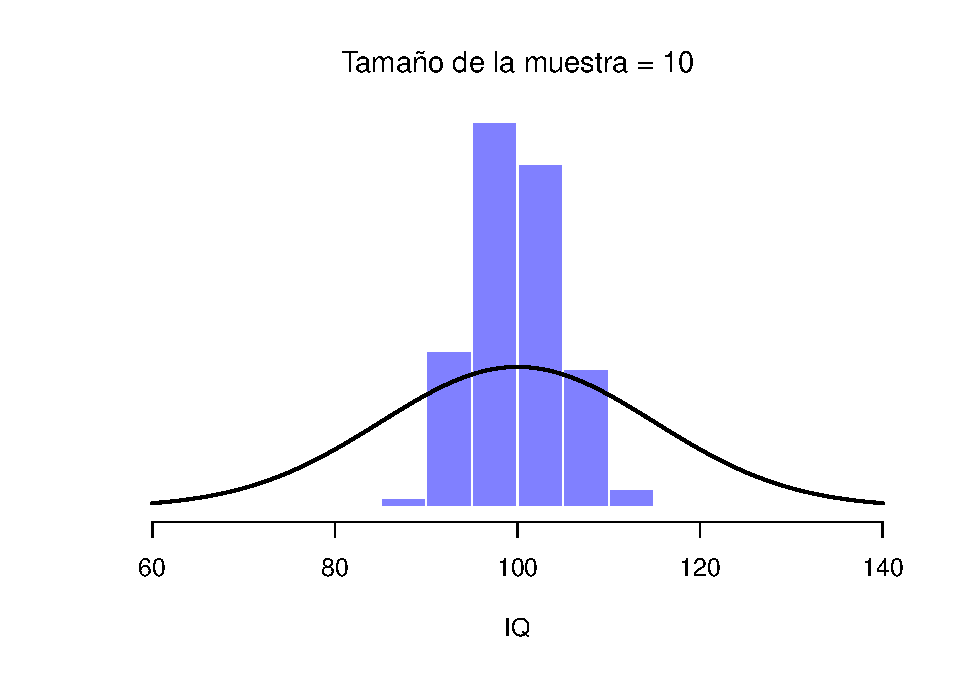
\includegraphics{FdI2_files/figure-latex/IQsampc-1.pdf} Espero que con
esta demostración, tengas un mejor idea de lo que son las distribuciones
muestrales, y en particular lo que es la distribución muestral de la
media. En esta sección hablaremos de cómo la distribución muestral de la
media cambia en función del tamaño muestral. Intuitivamente tú ya
conoces la respuesta: si tenemos sólo unas cuantas observaciones, es
probable que la media muestral no sea muy precisa. Si replicas este
experimento con una muestra pequeña y vuelves a calcular la media
obtendrás, casi con seguridad, una respuesta muy diferente. En otras
palabras, su distribución muestral es muy ancha. Por otro lado, si
replicas un experimento con un tamaño muestral grande y calculas la
media muestral varias veces, es muy probable que obtengas la misma
respuesta, o al menos muy aproximada, por lo que la distribución
muestral será muy estrecha. Esto lo puedes apreciar visualmente con las
Figuras \ref{fig:IQsampa}, \ref{fig:IQsampb} y \ref{fig:IQsampc}: entre
más grande sea la muestra, más estrecha será la distribución muestral.
Podemos cuantificar este efecto si calculamos la desviación estándar de
la distribución muestral, mejor conocida como el \textbf{\emph{error
estándar}}. El error estándar de la media se denota como \(\sigma\) con
el subíndice \(\bar{X}\) (o SEM en inglés). Y como puedes ver y
confirmar con las figuras, conforme aumenta el tamaño muestral \(N\), el
error estándar disminuye.

De momento hemos visto cómo se comportan las distribuciones muestrales
de los puntajes de CI, que es un parámetro que tiene una distribución
poblacional normal. Pero, ¿qué pasa con aquellos datos que no guardan
una distribución normal? Esta es la clave: sin importar la forma de la
distribución de la población, si aumentamos \(N\), su distribución
muestral siempre será como la que hemos visto con la distribución
normal. Por ejemplo, en la Figura \ref{fig:cltdemo} verás que una
distribución poblacional que tiene forma de rampa (los valores más altos
son los más frecuentes). Si comparas esta forma con la de la
distribución normal (la línea sólida negra), podrás confirmar que no se
parecen en nada. Si repetimos el mismo procedimiento que hemos hecho
anteriormente, y extraemos un número elevado de muestras (10,000) con un
tamaño muestral de \(N=2\) y calculamos sus medias muestrales,
obtendremos la distribución muestral de la media que puedes ver en la
Figura \ref{fig:cltdemob}. Esta distribución cambia de forma de manera
importante, y aunque no es normal, se aproxima bastante, sobre todo si
la comparamos con la distribución poblacional original (Figura
\ref{fig:cltdemoa}). Si aumentamos el tamaño muestral a \(N=4\), la
distribución muestral de la media se acerca más a una distribución
normal (Figura \ref{fig:cltdemoc}, y con un tamaño muestral de \(N=8\)
esta ya es perfectamente normal. En otras palabras, siempre y cuando el
tamaño de tu muestra no sea diminuto, la distribución muestral de la
media será normal, ¡sin importar la forma de la distribución
poblacional!

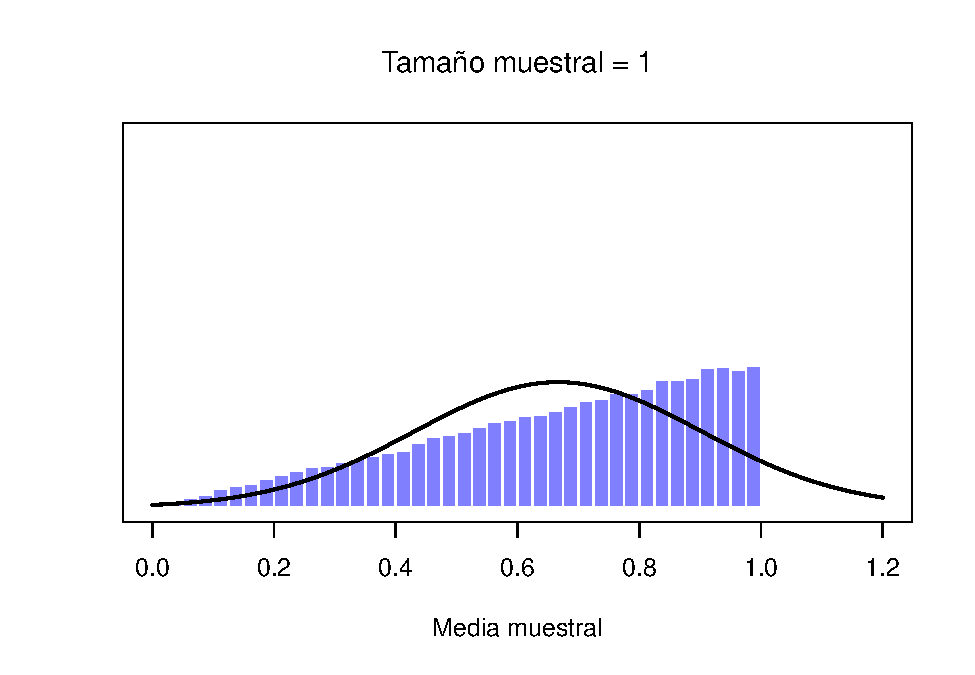
\includegraphics{FdI2_files/figure-latex/cltdemo-1.pdf}
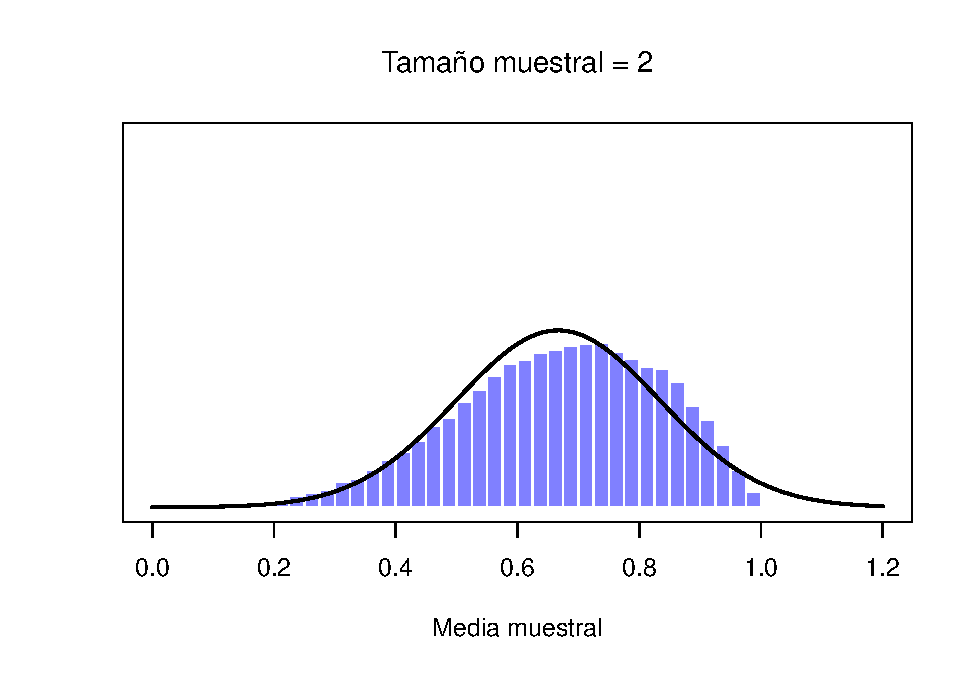
\includegraphics{FdI2_files/figure-latex/cltdemo-2.pdf}
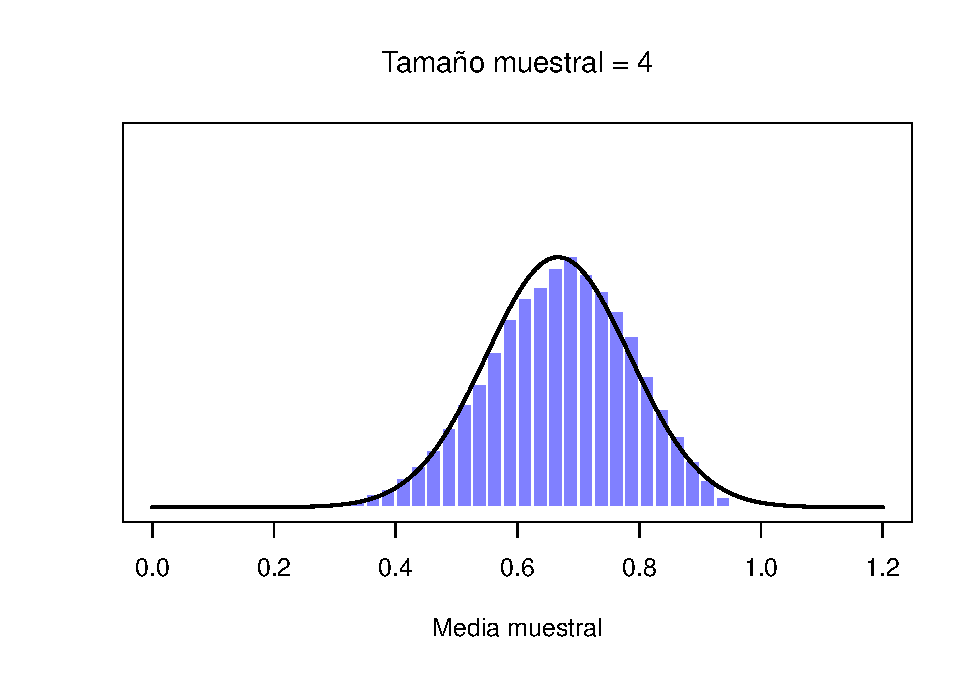
\includegraphics{FdI2_files/figure-latex/cltdemo-3.pdf}
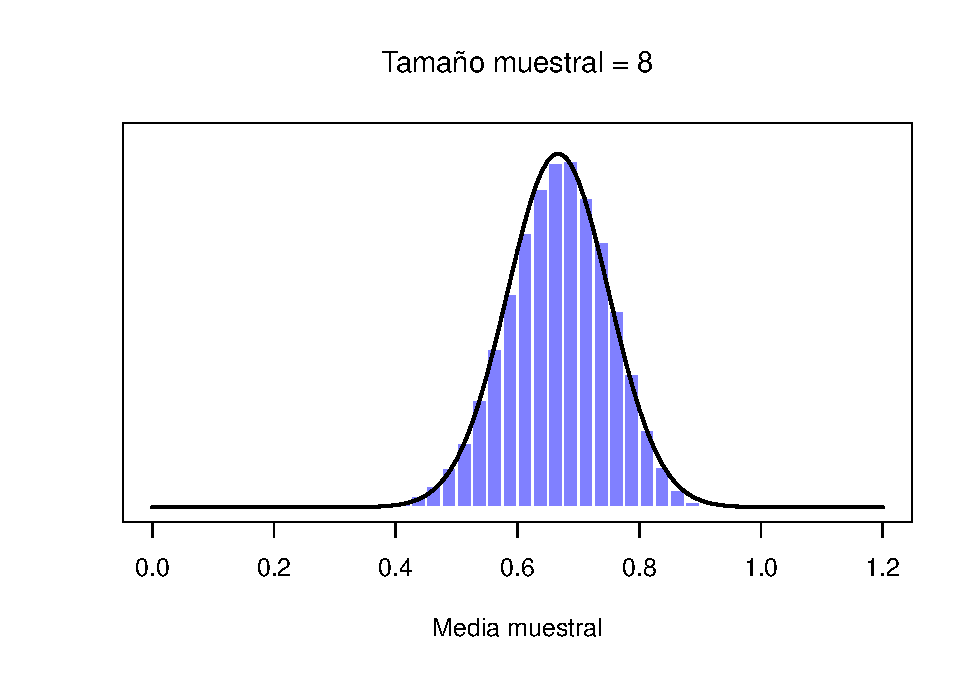
\includegraphics{FdI2_files/figure-latex/cltdemo-4.pdf}

Con base en estas figuras, parece que tenemos evidencia suficiente para
sustentar las siguientes afirmaciones sobre las distribuciones
muestrales de la media:

\begin{itemize}
\tightlist
\item
  La media de una distribución muestral es igual a la media poblacional
\item
  La desviación estándar de una distribución muestral (el error
  estándar) disminuye conforme aumenta el tamaño muestral
\item
  La forma de una distribución muestral adquiere una forma normal o de
  campana conforme aumenta el tamaño muestral
\end{itemize}

Estas tres afirmaciones que hemos deducido, pueden ser comprobadas a
través de un teorema muy famoso en estadística, conocido como el
\textbf{\emph{teorema del límite central}}. Entre otras cosas, el
teorema del límite central nos dice que si una distribución poblacional
tiene una media \(\mu\) y una desviación estándar \(\sigma\), entonces
la distribución muestral de la media también tendra una media \(\mu\) y
un error estándar de la media:

\[
\mbox{SEM} = \frac{\sigma}{ \sqrt{N} }
\] Ya que en esta fórmula se divide la desviación estándar de la
población \(\sigma\) por la raíz cuadrada del tamaño muestral \(N\), el
error estándar disminuye conforme aumenta el tamaño muestral. También
nos dice que la forma de la distribución muestral se vuelve normal.
\footnote{Hemos explicado el caso de la media muestral que satisface el
  teorema del límite central. Sin embargo, existen otros estadísticos
  muestrales que también lo hacen, y que no revisaremos, al ser esto una
  introducción.}

Este resultado es útil por muchas razones. Nos dice porqué los
experimentos con un tamaño muestral más grande son más confiables que
aquellos con muestras pequeñas, además de darnos una fórmula para el
error estándar que nos permite cuantificar \emph{qué tanto} más
confiable es ese experimento. Nos dice que porque la distribución
normal, es\ldots{} \emph{normal}. Cuando hacemos un experimento, muchas
de las cosas que medimos son en realidad un promedio de muchas otras
medidas (por ejemplo, la inteligencia ``general'' que mide el CI es un
promedio de un gran número de habilidades ``específicas''), y cuando eso
pasa, la cantidad promediada debe seguir una distribución normal. Es por
esta ley matemática que la distribución normal aparace con tanta
frecuencia en los datos que recogemos del mundo real.

\section{Estimando parámetros poblacionales}\label{pointestimates}

En todos los ejemplos anteriores sobre el CI, hemos asumido que
conocíamos los parámetros poblacionales. Los tests que miden el CI están
\emph{diseñados} para tener una media de 100 y una desviación estándar
de 15: cuando se estudia el CI en una población, se obtienen datos de
una muestra muy grande y después se ``ajustan'' los resultados de forma
que la media sea de 100. Esto nos sirve para recordar que una media es
representativa únicamente de su población. En ocasiones podremos
encontrar ``normas'' que permiten aplicar esos parámetros en otras
poblaciones diferentes (por ejemplo, grupos de edad diferente,
nacionalidades, etc.).

Supongamos que ahora queremos explorar el efecto que tiene la
contaminación ambiental en el rendimiento académico a través del CI.
Para ello obtendremos y compararemos los puntajes de CI de estudiantes
de una ciudad con altos índices de contaminación -Albacete- y otra con
baja contaminación ambiental -Vitoria- (evidentemente, existen muchos
otros factores que pueden influir en el puntaje final de CI).
Independientemente de la ciudad que escojamos, no podemos \emph{asumir}
que la media de su población es de 100. No se ha creado una ``norma''
que se aplique al nivel de contaminación ambiental de las ciudades y su
relación con el CI. Por ello, tendremos que \textbf{\emph{estimar}} los
parámetros de la población a partir de una muestra.

\subsection{Estimando la media
poblacional}\label{estimando-la-media-poblacional}

Supongamos que vamos a Albacete y conseguimos los puntajes de CI de una
muestra de 100 amables albaceteños. Obtenemos que el puntaje medio de
esas personas es de \(\bar{X}=98.5\). Entonces, ¿cuál la media real del
CI para la población entera de Albacete? Evidentemente, no conocemos la
respuesta a esa pregunta. Podría ser \(97.2\), pero también \(103.5\).
Nuestra muestra no es lo suficientemente grande como para darnos una
respuesta definitiva. Sin embargo, si tuviera que apostar, diría que es
\(98.5\). Esta es la esencia de la estimación estadística: dar tu mejor
predicción.

En este ejemplo, estimar este parámetro de la población es muy sencillo.
Calculamos la media muestral, y utilizo este mismo resultado como el
\textbf{\emph{estimador de la media poblacional}}. En la siguiente
sección explicaré la justificación estadística para esta respuesta que
parece intuitiva. Por lo pronto, lo que debes reconocer es que,
conceptualmente, la media muestral y el estimador de la media
poblacional son cosas diferentes. Un estadístico muestral es una
descripción de los datos, mientras que un estimador es una predicción
sobre la población. Con esto en mente, los estadísticos utilizan una
notación diferente para referirse a cada una de ellas. Así, mientras que
la media poblacional se denota como \(\mu\), el estimador de la media
poblacional utiliza \(\hat\mu\) (recuerda que para referirnos a la media
muestral usamos \(\bar{X}\)). Sin embargo, en muestras simples
aleatorias, el estimador de la media poblacional es idéntico a la media
muestral: si obtenemos una media muestral de \(\bar{X} = 98.5\),
entonces mi estimador de la media poblacional será también de
\(\hat\mu = 98.5\). Esta tabla nos ayudará a guardar el registro:

\begin{tabular}{l|l|l}
\hline
Simbolo & Valor & Lo.conocemos\\
\hline
\$\textbackslash{}bar\{X\}\$ & Media muestral & Sí, lo calculamos a partir de datos\\
\hline
\$\textbackslash{}mu\$ & Media poblacional & Casi nunca\\
\hline
\$\textbackslash{}hat\{\textbackslash{}mu\}\$ & Estimador de la media poblacional & Sí, idéntico a la media muestral\\
\hline
\end{tabular}

\subsection{Estimando la desviación estándar
poblacional}\label{estimando-la-desviacion-estandar-poblacional}

De momento, la estimación parece algo sencillo, por lo que te
preguntarás porqué te hecho leer todo eso sobre la teoría de muestreo.
En el caso de la media, nuestro estimador de la media poblacional
\(\hat\mu\) resulta ser idéntico a la media muestral \(\bar{X}\). Sin
embargo, esto no aplica para todos los estadísticos muestrales. Como
ejemplo, veamos como se construye el \textbf{\emph{estimador de la
desviación estándar poblacional}}, cuya notación es \(\hat\sigma\). Si
seguimos el mismo razonamiento que con el estimador de la media
poblacional \(\hat\mu\), cogeríamos a la desviación estándar muestral
como nuestro estimador. Esto nos dará una respuesta aproximadamente
correcta, pero no del todo.

Veamos porqué. Supongamos que tenemos una muestra de puntajes de CI que
contiene una única observación. Este único puntaje es de 99, por lo que
tendremos la siguiente muestra:

\begin{verbatim}
99
\end{verbatim}

Esta es una muestra perfectamente legítima, aunque tenga un tamaño de
muestra de \(N=1\). Esta muestra tiene una media de 99, y al no haber
ninguna otra observación en esta muestra, no existe dispersión de datos
y por lo tanto tenemos una desviación estándar muestral de 0. Como
descripción de una \emph{muestra} esto es válido: la muestra contiene
una sola observación y por lo tanto no hay variabilidad o dispersión
dentro de la muestra. En este caso, decir que tenemos una desviación
estándar muestral de \(s = 0\) es correcto. Pero si utilizamos este
valor como estimador de la desviación estándar \emph{poblacional} parece
no tener sentido. No vemos variabilidad en esta \emph{muestra}
simplemente porque ¡la muestra es tan pequeña que no puede mostrar
variabilidad! Por lo tanto, si tenemos un tamaño muestral de \(N=1\),
``no tenemos ni idea'' del estimador de la desviación estándar
poblacional.

Observa como en este caso \emph{no} has tenido la misma intuición que
con la media muestral y su estimador. Aunque tengamos una media de 99 a
partir de una única observación, es un valor \emph{plausible}, y nos
permite al menos, hacer una predicción.

Vamos a dar un paso más en este ejemplo. Supongamos que ahora recolecto
una segunda observación. Mi muestra tiene ahora \(N=2\) puntajes de CI,
que son los siguientes:

\begin{verbatim}
99, 101
\end{verbatim}

Esta vez, la muestra es lo \emph{suficientemente} grande para que
podamos observar algo de variabilidad en ella: dos observaciones es el
número mínimo necesario para observar cualquier variabilidad. Para esta
nueva muestra, la media muestral es de \(\bar{X}=100\), y su desviación
estándar es de \(s=1\). ¿Qué intuiciones o suposiciones podemos hacer de
la población? Nuevamente, la mejor predicción que podemos hacer es con
la media muestral: si tuviéramos que adivinar, diríamos que la media
poblacional es de 100. ¿Y que hay de la desviación estándar? Aquí es un
poco más complicado. La desviación estándar muestral está basada
únicamente en dos observaciones, y es probable que con esto no hemos
dado a la población ``suficiente oportunidad'' para mostrar cual es su
variabilidad real. No es que simplemente sospechemos que utilizar este
valor como estimador sea un \emph{error}: después de todo, con dos
observaciones esperamos que \emph{esté} equivocado en cierto grado. El
problema es que este error sea \emph{sistemático}. Específicamente,
sospechamos que la desviación estándar muestral sea menor que desviación
estándar poblacional.

\begin{figure}
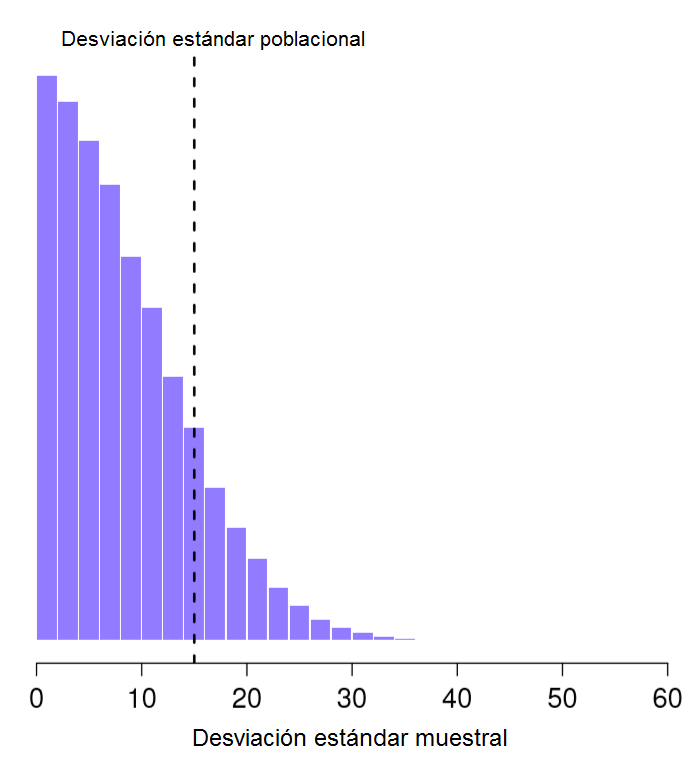
\includegraphics[width=9.65in]{img/estimation/samplingDistSampleSD} \caption{Distribución muestral de la desviación estándar del experimento con "dos puntajes de CI". La media real poblacional es de 15 (línea punteada), pero como puedes ver en el histograma, la mayor parte de los experimentos producirán un valor de desviación estándar muestral mucho más pequeño. En promedio, este experimento daría como resultado una desviación estándar muestral de sólo 8.5, muy por debajo del valor real. En otras palabras, la desviación estándar muestral es un estimador *sesgado* de la desviación estándar poblacional.}\label{fig:sampdistsd}
\end{figure}

Aunque esta intuición pueda ser correcta, sería importante poder
demostrarla. Si calculamos \emph{la distribución muestral de la
desviación estándar} para nuestro experimento de \(N=2\) puntajes de CI,
veremos que el promedio de esas distribuciones estándar
\emph{muestrales} es de tan sólo 8.5 (puedes ver esta distribución en la
Figura \ref{fig:sampdistsd}), muy por debajo de la desviación estándar
poblacional de 15. Observa que esta distribución es muy diferente a la
distribución muestral de la media que vimos en la Figura
\ref{fig:IQsampb}. En ella, la media poblacional es de 100, y el
promedio de las medias muestrales también es de 100.

Ahora extendamos un poco más esta simulación. En lugar de limitarnos a
calcular la distribución muestral de la desviación de muestras de tamaño
\(N=2\), repitamos este ejercicio con tamaños muestrales del 1 al 10. Si
graficamos como cambia el promedio de las medias muestrales y las
desviaciones estándar muestrales en función del tamaño muestral,
obtendremos lo que se enseña en la Figura \ref{fig:estimatorbias}. En la
parte izquierda (a) vemos graficada los promedios de las medias
muestrales y en la parte izquierda los promedios de las desviaciones
estándar. Ambas gráficas son diferentes: \emph{en promedio}, la media
muestral es igual a la media poblacional. Esto lo convierte en un
\textbf{\emph{estimador insesgado}}, y es el motivo por el cual la media
muestral es el mejor estimador de la media poblacional. En la parte
derecha (b), vemos una gráfica distinta: \emph{en promedio}, la
desviación estándar muestral \(s\) es \emph{menor} que la desviación
estándar poblacional \(\sigma\). Esto lo convierte en un
\textbf{\emph{estimador sesgado}}. En otras palabras, si queremos hacer
nuestra mejor ``predicción'' \(\hat\sigma\) del valor de la desviación
estándar poblacional \(\sigma\), podríamos hacerlo aumentando el tamaño
de la desviación estándar muestral \(s\).

\begin{figure}
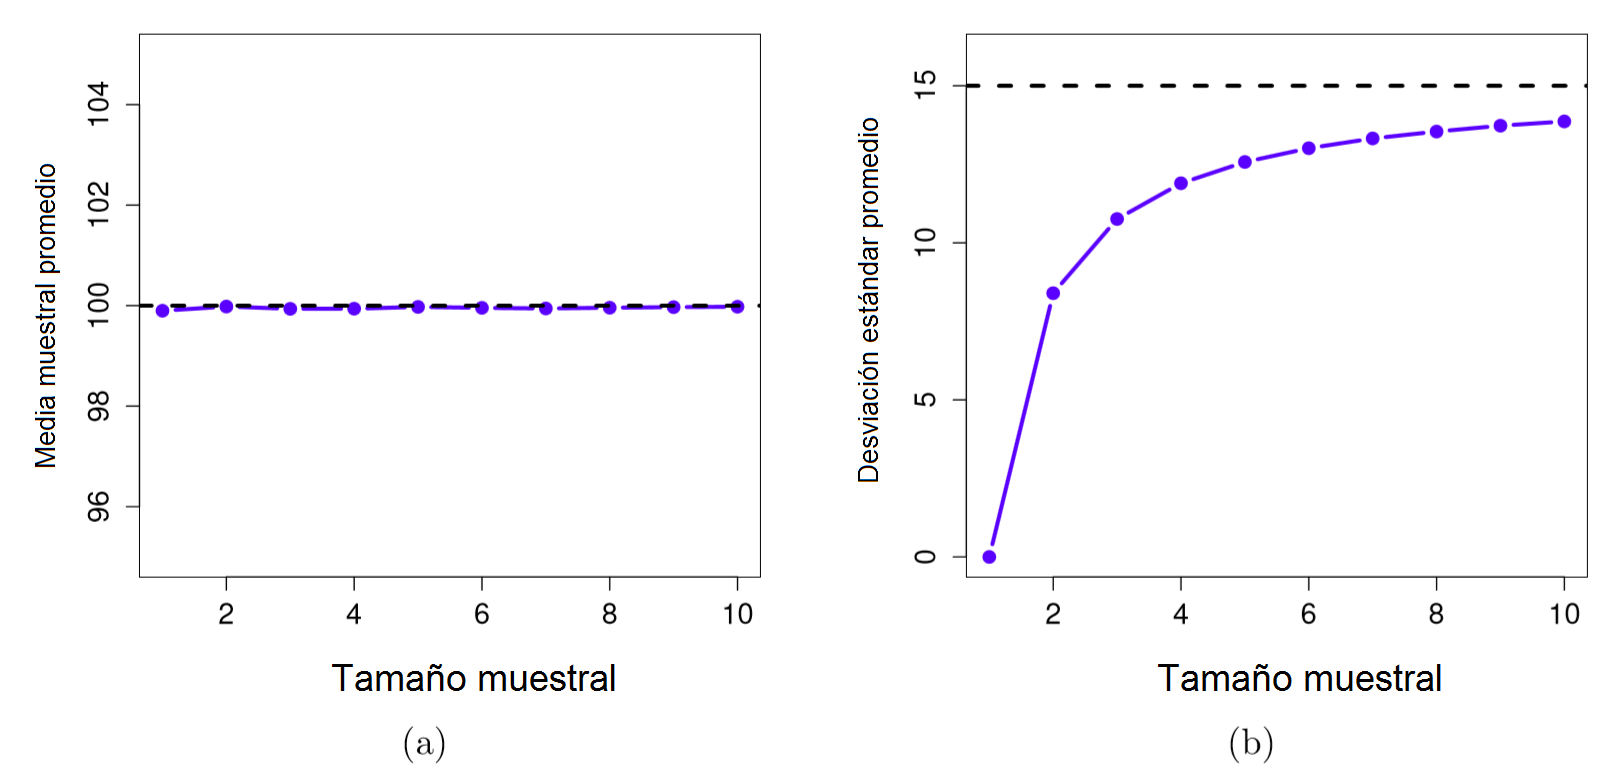
\includegraphics[width=22.4in]{img/estimation/biasMeanSD} \caption{Demostración del hecho de que la media muestral es un estimador insesgado de la media poblacional (a), mientras que la desviación estándar es un estimador sesgado de la desviación estándar poblacional (b). *En promedio*, la media muestral es 100, independientemente del tamaño muestral (a). Sin embargo, la desviación estándar muestral es sistemáticamente menor que la desviación estándar poblacional (b), sobre todo con tamaños de muestra pequeños.}\label{fig:estimatorbias}
\end{figure}

Arreglar este error sistemático es muy sencillo. Primero, recordemos la
fórmula de la desviación estándar poblacional: \[
\sigma = \sqrt\frac{\sum_{i=1}^N (X_i - \bar{X})^2}{N} 
\] Sólo hace falta un pequeño cambio para corregir ese error
sistemático. Lo único que tenemos que hacer dividir por \(N-1\) en lugar
de por \(N\). Si lo hacemos, obtendremos la siguiente fórmula: \[
\hat\sigma = \sqrt\frac{\sum_{i=1}^N (X_i - \bar{X})^2}{N-1} 
\] Un último apunte: en la práctica, mucha gente se refiere a
\(\hat{\sigma}\) (esta última fórmula) como la desviación estándar
\emph{muestral}. Técnicamente, esto es incorrecto: en la desviación
estándar \emph{muestral} se divide únicamente por \(N\). Y es que no son
lo mismo, ni conceptualmente ni numéricamente. Uno es una propiedad de
una muestra, mientras que el otro es una característica estimada de la
población. Sin embargo, lo normal es que nos interesemos por calcular el
estimador de la población, por lo que solemos utilizar \(\hat\sigma\) en
lugar de \(s\). Quizás esta imprecisión se deba a que es más fácil
escribir ``desviación estándar muestral'' que ``estimador de la
desviación estándar poblacional''. En la práctica, no suele haber mucha
diferencia, sin embargo, es importante separar ambos \emph{conceptos}:
no debemos confundir las ``características conocidas de tu muestra'' con
las ``predicciones acerca de la población''.

\begin{tabular}{l|l|l}
\hline
Simbolo & Valor & Lo.sabemos\\
\hline
\$s\$ & Desviación estándar muestral & Sí, lo calculamos a partir de datos\\
\hline
\$\textbackslash{}sigma\$ & Desviación estándar poblacional & Casi nunca\\
\hline
\$\textbackslash{}hat\{\textbackslash{}sigma\}\$ & Estimador de la desviación estándar poblacional & Sí, pero no es igual a la desviación estándar muestral\\
\hline
\end{tabular}

\section{Estimando un intervalo de confianza}\label{ci}

Hasta este punto en esta 2ª Unidad, hemos revisado los conceptos básicos
de la teoría de muestreo que los estadísticos utilizan para hacer
predicciones sobre los parámetros poblacionales a partir de una muestra
de datos. Una de las razones por las cuales necesitamos de esta teoría
de muestro es que cada conjunto de datos nos deja con un cierto grado de
incertidumbre, por lo que nuestros estimadores nunca serán precisos a la
perfección. Sin embargo, nosotros somos capaces de \emph{cuantificar}
esa incertidumbre que va implícita en nuestros estimadores. No basta con
predecir que el CI medio de mi muestra de estudiantes es de 105; también
podemos expresar el grado de certeza que tenemos sobre esa predicción.\\
Nos gustaría, por ejemplo, decir que tenemos un 95\% de probabilidad de
que un rango de valores contenga la media real. Esta herramienta existe
y recibe el nombre de \textbf{\emph{intervalo de confianza}} de la
media.

Como ya conocemos y entendemos como funcionan las distribuciones
muestrales, construir un intervalo de confianza resulta relativamente
sencillo. Supongamos que la media real poblacional es \(\mu\) y la
desviación estándar es \(\sigma\). Hemos terminado un estudio que
incluye a \(N\) participantes, y el CI medio de esos participantes es de
\(\bar{X}\). Por nuestra discusión sobre teorema del límite central
(Sección \ref{clt}), sabemos que la distribución muestral de la media es
aproximadamente normal. También sabemos por nuestra discusión sobre la
distribución normal (Sección \ref{normal}) que existe un 95\% de
probabilidad de que una cantidad normalmente distribuida caiga dentro de
dos desviaciones estándar alrededor de la media real (es decir, entre
los percentiles 2.5 y 97.5). Aunque si vamos al detalle (con la ayuda de
nuestra tabla z), vemos que no son dos desviaciones estándar
exactamente, sino 1.96, que es el número que utilizaremos de aquí en
adelante.

Ahora, recordemos que cuando hablamos de la desviación estándar de una
distribución muestral, nos estamos refiriendo al error estándar, en este
caso, de la media (SEM). Si juntamos todos estos elementos, podemos
decir que existe una probabilidad del 95\% de que la media muestral
\(\bar{X}\) caiga dentro de 1.96 desviaciones estándar de la media
poblacional. Matemáticamente lo podemos expresar de la siguiente forma:
\[
\mu - \left( 1.96 \times \mbox{SEM} \right) \ \leq \  \bar{X}\  \leq \  \mu + \left( 1.96 \times \mbox{SEM} \right) 
\] donde el error estándar (SEM) es igual a \(\sigma / \sqrt{N}\). Sin
embargo, esto no responde a nuestra pregunta original. La ecuación
anterior nos dice lo que podemos esperar de la media muestral, dado que
conocemos los parámetros poblacionales. En cambio, lo que nosotros
\emph{queremos} saber es justo lo contrario: queremos conocer qué creer
de los parámetros poblacionales, dado lo observado a partir de una
muestra. Por lo tanto, podemos aplicar nuestros conocimientos de álgebra
y despejar esta ecuación de forma que nos de la respuesta que buscamos:
\[
\bar{X} -  \left( 1.96 \times \mbox{SEM} \right) \ \leq \ \mu  \ \leq  \ \bar{X} +  \left( 1.96 \times \mbox{SEM}\right)
\] Lo que esta nueva ecuación nos dice, es que un rango de valores tiene
un 95\% de probabilidad de contener la media poblacional \(\mu\). A este
rango específico lo conocemos como el \textbf{\emph{intervalo de
confianza de 95\%}}, y se denota como \(\mbox{CI}_{95}\). Así, mientras
el tamaño de muestra \(N\) sea lo suficientemente grande
-suficientemente grande para creer que la distribución muestral de la
media es normal-, entonces podemos escribir nuestra fórmula del
intervalo de confianza de 95\% de la siguiente forma: \[
\mbox{CI}_{95} = \bar{X} \pm \left( 1.96 \times \frac{\sigma}{\sqrt{N}} \right)
\] Es imporante aclarar que no hay nada de especial en el número 1.96;
simplemente es el multiplicador para un nivel de confianza del 95\% que
suele ser el más utilizado cuando se calcula un intervalo de confianza.
Dependiendo de las circunstancias, podemos disminuir o aumentar ese
nivel de confianza (por ejemplo, un nivel de confianza de 70\% nos da un
valor de 1.04).

\subsection{¿Qué pasa cuando no conocemos los parámetros
poblacionales?}\label{que-pasa-cuando-no-conocemos-los-parametros-poblacionales}

La fórmula que hemos utilizado para calcular el intervalo de confianza
de 95\% es aproximadente correcta. Sin embargo, no hemos explorado un
detalle importante dentro de esta discusión. La fórmula requiere que
usemos el error estándar de la media (SEM), que a su vez requiere que
utilicemos la desviación estándar de la población \(\sigma\). No
obstante, en la Sección \ref{pointestimates} vimos que, por lo general,
nosotros no \emph{conocemos} los parámetros poblacionales. Como no
conocemos el valor verdadero de \(\sigma\), tenemos que usar el
estimador de la desviación estandar \(\hat{\sigma}\) en su lugar. Esto
tiene como consecuencia que tenemos que usar los cuantiles de la
distribución \(t\) en lugar de los de la distribución normal (valores
\(z\)); y la elección de ese cuantil depende directamente del tamaño
muestral. Si la \(N\) es muy grande, obtendremos prácticamente el mismo
valor: para un nivel de confianza del 95\%, una muestra de tamaño
\(N=10,000\), nos da un valor \(t\) de 1.96. Pero si la \(N\) es pequeña
obtendremos un valor \(t\) mucho mayor: utilizando el mismo nivel de
confianza, pero una muestra con \(N=10\), el valor \(t\) es igual a
2.26.

Un valor más grande nos dice que el intervalo de confianza es más ancho,
lo cual indica mayor incertidumbre sobre dónde se encuentra la media
real poblacional \(\mu\). Cuando utilizamos la distribución \(t\) en
lugar de la distribución normal, obtenemos números más grandes, lo que
indica un mayor grado de incertidumbre. ¿Y esto a que se debe? Se debe
simplemente a que el estimador de la desviación estándar poblacional
\(\hat\sigma\) puede estar equivocado. Si está equivocado, implica que
estamos un poco menos seguros sobre la forma de la distribución muestral
de la media\ldots{} y esta incertidumbre se ve reflejada en un intervalo
de confianza más ancho.

\subsection{Interpretando un intervalo de
confianza}\label{interpretando-un-intervalo-de-confianza}

Quizás lo más difícil sobre un intervalo de confianza es entender lo que
en realidad \emph{significa}. Cuando vemos por primera vez un intervalo
de confianza, el primer instinto es decir ``que existe un probabilidad
del 95\% de que la media real se encuentre dentro del intervalo de
confianza''. Sin embargo, esta idea que parece acorde con el sentido
común, está equivocada. Esta definición confía fuertemente en las
\emph{creencias} personales sobre el valor de la media poblacional: ``yo
creo que este valor tiene un 95\% de probabilidad de entrar en este
rango''. Si recuerdas lo que vimos en la Sección \ref{probmeaning}, te
darás cuenta que cuando hablamos de creencias personales y confianza,
estamos hablando de la estadística Bayesiana. Sin embargo, los
intervalos de confianza \emph{no} son herramientas Bayesianas. Como casi
todo lo que hemos visto en este curso, los intervalos de confianza son
herramientas \emph{frecuentistas}, y como tal, debemos adoptar
interpretaciones frecuentistas.

Revisemos el concepto de probabilidad frecuentista: para poder hacer
declaraciones de probabilidad, tenemos que referirnos a una serie de
eventos, y contar las frecuencias de los diferentes tipos de eventos
(como cuando lanzamos muchas veces una moneda y contamos el número de
caras y de cruces). Desde esta perspectiva, la interpretación del
intervalo de confianza de 95\% tendrá que ver con la repetición de
experimentos o replicación: si replicamos el experimento una y otra vez
y calculamos el intervalo de confianza del 95\% para cada replicación,
entonces el 95\% de esos \emph{intervalos} contendrán la media real
poblacional. Esta idea se ilustra en la Figura \ref{fig:cirep}, que
muestra 50 intervalos de confianza construidos para un ``experimento que
mide 10 puntajes de CI'' y otros 50 intervalos de confianza para un
``experimento que mide 25 puntajes de CI''. En este ejemplo, vemos como
exactamente el 95\% de los intervalos de confianza contiene a la media
real.

\textbackslash{}begin\{figure\}
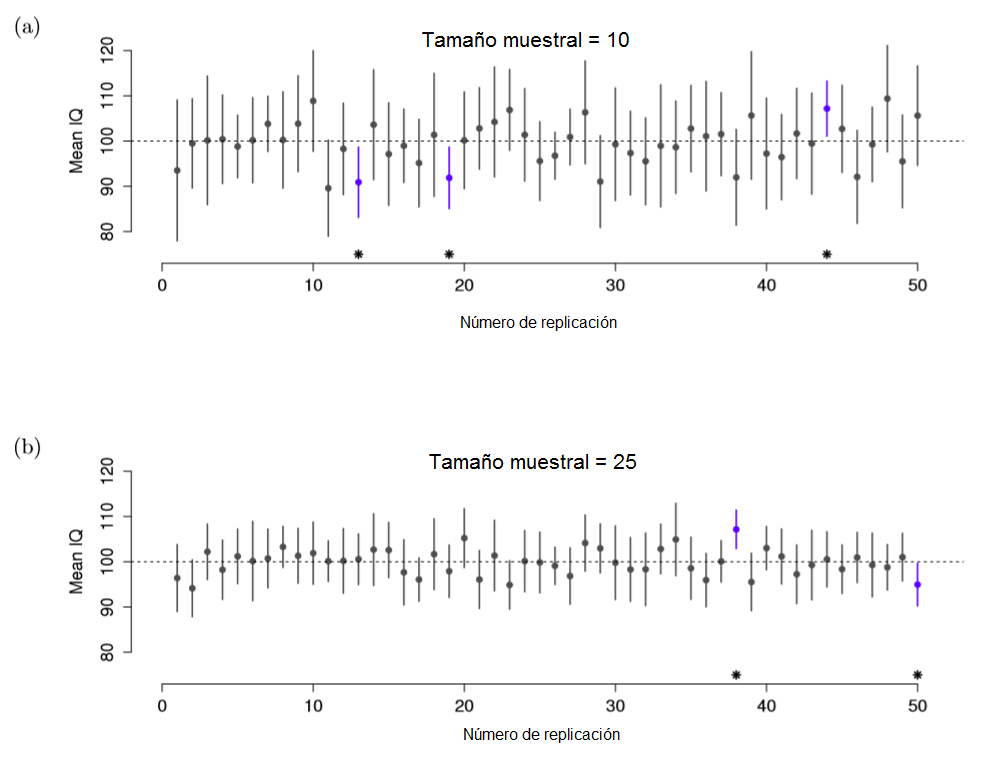
\includegraphics[width=13.75in]{img/estimation/confIntReplicated}
\textbackslash{}caption\{Intervalos de confianza de 95\%. En la parte
superior (a) se muestran 50 replicaciones de un experimento que mide el
CI de 10 personas. Los puntos indican la localización de la media
muestral, y las líneas indican el intervalo de confianza de 95\%. En un
47 de 50 replicaciones, el intervalo de confianza contiene a la media
real poblacional (i.e.~100), mientras que tres intervalos no la
contienen (marcados con un asterisco). En la parte inferior (b) se
muestra una simulación similar, pero con la replicación de un
experimento que mide el CI de 25 personas. Observa con los intervalos de
confianza son más pequeños con muestras más grandes.\}\label{fig:cirep}
\textbackslash{}end\{figure\}

La diferencia clave es que la pretensión Bayesiana es hacer una
declaración de probabilidad sobre la media poblacional, lo cual no está
permitido bajo una interpretación de la probilidad frecuentista ya que
no se puede ``replicar'' una población. Desde el punto de vista
frecuentista, la media poblacional es fija y no se pueden hacer
declaraciones de probabilidad sobre ella. Sin embargo, los intervalos de
confianza sí que son repetibles, y por lo tanto, podemos replicar
experimentos. Así, un frecuentista puede hablar sobre la probabilidad de
que el \emph{intervalo de confianza} (una variable aleatoria) contenga
la media poblacional; pero no puede hablar sobre la probabilidad de que
la \emph{media real poblacional} (un evento no repetible) caiga dentro
de un intervalo de confianza.

\section{Estimando el tamaño muestral}\label{samplesize}

Hasta este punto, hemos aprendido a utilizar las herramientas que nos
permiten reducir el nivel de incertidumbre cuando queremos conocer los
parámetros de una población a partir de los resultados de una muestra.
Sabemos estimar un parámetro poblacional y establecer su intervalo de
confianza. También hemos aprendido, gracias a la ley de los grandes
números, que el \emph{grado de incertidumbre} depende particularmente
del tamaño de la muestra: mientras tengamos un mayor tamaño muestral,
los estimadores se aproximarán más a los parámetros reales poblacionales
y sus intervalos de confianza serán más estrechos.

Sin embargo, sabemos que en muchas ocasiones no podremos aspirar a un
tamaño muestral tan grande como los que hemos utilizados en nuestors
ejemplos. Es habitual que un investigador se vea limitado a recolectar
una muestra pequeña por motivos económicos, de accesibilidad, prácticos,
o porque simplemente no tiene el tiempo para ello. Por todo esto, espero
que entiendas la importancia que tiene calcular el tamaño de una muestra
que, nos de resultados de los que cuales nos podamos fiar, y a su vez,
no se convierta en una tarea imposible para el investigador.

Por suerte, calcularlo no es muy complicado y podemos reutilizar los
conceptos que hemos aprendido en esta Unidad. Para ello, tomemos nuestra
fórmula del intervalo de confianza de 95\%: \[
\mbox{CI}_{95} = \bar{X} \pm \left( 1.96 \times \frac{\sigma}{\sqrt{N}} \right)
\] Si te fijas bien, observarás que está fórmula necesita del tamaño
muestral \(N\) para poder ser resuelta. Para llegar a ella, podemos
empezar por separar los elementos que conforman a la fórmula del
intervalo de confianza (media muestral y margen de error), y quedarnos
con el \textbf{\emph{margen de error}} (\(ME\)) que es el resultado de
multiplicar el nivel de confianza (en este caso 1.96), por el error
estándar: \[
ME = 1.96 \times \frac{\sigma}{\sqrt{N}} \
\] A partir de aquí, calcular \(N\) es muy sencillo. Si conocemos el
resto de elementos que integran la ecuación, podemos despejar \(N\) y
obtener la siguiente fórmula para el cálculo del \textbf{\emph{tamaño
muestral}}: \[
N = \left( 1.96 \times \frac{\sigma}{ME} \right)^2
\] Al observar esta fórmula, vemos que nos enfrentamos al mismo problema
que tuvimos al calcular el intervalo de confianza: en muchas ocasiones
no podremos conocer el valor de la desviación estándar poblacional
\(\sigma\). Adicionalmente, tampoco sabemos cuál es nuestro margen de
error (\(ME\)).

Para resolver el problema con la desviación estándar \(\sigma\) contamos
con dos opciones. Por un lado, podemos utilizar un valor de desviación
estándar \emph{aproximado}, que puede estar basado en los hallazgos
encontrados en poblaciones similares a nuestra población de interés, en
la teoría o puede ser simplemente un cálculo conservador que denote el
grado de incertidumbre que realmente tenemos sobre esa población. Por
otro lado, podemos llevar a cabo un \textbf{\emph{estudio piloto}}, en
el cual recolectemos los datos de una muestra pequeña que nos permitan
estimar un media \(\bar{X}\) y una desviación estándar muestrales \(s\)
que después podamos utilizar en el cálculo del tamaño muestral para un
estudio más grande.

En el caso del margen de error, la solución es un poco más fácil. Así
como el nivel de confianza que se utiliza con más frecuencia es el del
95\%, podemos aplicar este mismo criterio para el \(ME\). En
investigación se suele utilizar un margen de error de entre el 3\% y el
10\%, dependiendo de la necesidad o importancia de tener resultados más
o menos precisos. Una buena regla general, es utilizar el \textbf{5\% de
la media} como margen de error. De esta forma, aseguramos que los
intervalos de confianza que obtengamos a partir de esa muestra sean
estrechos y nos permitan esgrimir conclusiones con mayor seguridad.

\section{Resumen}\label{resumen-1}

En esta Unidad hemos cubierto dos grandes temas. En la primera mitad,
hablamos sobre la teoría de muestreo, y en la segunda hemos visto cómo
podemos usar la teoría de muestreo para construir estimadores de los
parámetros poblacionales. El contenido lo podemos organizar en las
siguientes ideas:

\begin{itemize}
\tightlist
\item
  Ideas básicas sobre las muestras, muestreo y poblaciones (Sección
  \ref{srs})
\item
  Teoría estadística del muestreo: la ley de los grandes números
  (Sección \ref{lawlargenumbers}), las distribuciones muestrales y el
  teorema del límite central (Sección \ref{samplesandclt}).
\item
  Estimar medias y desviaciones estándar (Sección \ref{pointestimates})
\item
  Estimar intervalos de confianza (Sección \ref{ci})
\item
  Estimar el tamaño muestral (Sección \ref{samplesize})
\end{itemize}

\bibliography{book.bib,packages.bib}


\end{document}
